% --------------------------------------------------------------------
% --------------------------------------------------------------------
% Modelo de Trabalho Acadêmico (tese de doutorado, dissertação de
% mestrado) em conformidade com 
% --------------------------------------------------------------------
% --------------------------------------------------------------------

% Opção	Efeito no Documento
% qualificacao =	Formata para monografia de qualificação
% mestrado	 = Dissertação de mestrado
% doutorado	 = Tese de doutorado (padrão)
% pre-defesa	 = Versão para apresentação à banca
% pos-defesa	 = Versão final do trabalho
% impressao	 = Versão para impressão (desativa capa em PDF)

\documentclass[mestrado,pre-defesa]{packages/ppg-ieee}

\usepackage[numbers]{natbib}
\bibliographystyle{ieeetr}



% --------------------------------------------------------------------
% Pacotes Opcionais
% --------------------------------------------------------------------
\usepackage{rotating}           % Usado para rotacionar o texto
\usepackage[all,knot,arc,import,poly]{xy}   % Pacote para desenhos gráficos
% Este pacote pode conflitar com outros pacotes gráficos como o ``pictex''
% Então é necessário usar apenas um dos pacotes conflitantes
\newcommand{\VerbL}{0.52\textwidth}
\newcommand{\LatL}{0.42\textwidth}

% --------------------------------------------------------------------

% ---
% Informações de dados para CAPA e FOLHA DE ROSTO
% ---
% Tanto na capa quanto nas folhas de rosto apenas a primeira letra da primeira palavra (ou nomes próprios) devem estar em letra maiúscula, todas as demais devem ser em letra minúscula.
\tituloPT{Aplicação de inteligência artificial para previsão de enchentes e mitigação de impactos nas comunidades costeiras}
\tituloEN{Application of artificial intelligence for flood prediction and impact mitigation in coastal communities}
\autor[Silva, D. W. S.]{Daiane Wan-Dall Splitter da Silva}
\genero{F} % Gênero da autora (M = Masculino / F = Feminino)
\orientador[Orientador]{Prof. Dr.}{Rodrigo Sant'Ana}
% \coorientador{Prof. Dr.}{Nome do Coorientador} % descomente se houver coorientação
\curso{PPGC}
\data{20}{10}{2026} % Data do depósito (ajuste na entrega)
\idioma{PT} % Idioma principal do documento (PT = português / EN = inglês)
% ---

% ---
% RESUMOS
% ---

% Resumo em PORTUGUÊS
% conter no máximo 500 palavras
% conter no mínimo 1 e no máximo 5 palavras-chave
\textoresumo[brazil]{

Este projeto tem como objetivo o desenvolvimento de um modelo preditivo para a previsão de enchentes em comunidades costeiras do estado de Santa Catarina, utilizando técnicas avançadas de inteligência artificial. O aumento da frequência e da intensidade de eventos climáticos extremos, como chuvas intensas, marés elevadas e alagamentos, tem afetado diretamente a vida das populações litorâneas, ocasionando prejuízos sociais, ambientais e econômicos consideráveis. Nesse contexto, torna-se essencial a antecipação desses eventos, por meio de métodos mais precisos e eficazes do que os atualmente utilizados. A proposta deste trabalho é criar um sistema preditivo baseado na análise de dados ambientais, climáticos, hidrológicos e socioeconômicos, com foco na identificação de padrões e na projeção de cenários futuros de risco. Justifica-se a relevância da pesquisa pela possibilidade de oferecer uma ferramenta capaz de auxiliar a tomada de decisão por parte de autoridades e órgãos de proteção civil, promovendo maior segurança, planejamento urbano eficiente e proteção de áreas vulneráveis. A metodologia a ser adotada é de natureza aplicada, com abordagem quantitativa e método hipotético-dedutivo. O projeto incluirá a consolidação de um banco de dados estruturado com informações provenientes de sensores ambientais, imagens de satélite e registros históricos de enchentes. Serão aplicadas técnicas de aprendizado de máquina para o desenvolvimento, ajuste e validação dos modelos preditivos. Espera-se, como resultado, a criação de um modelo robusto e confiável, capaz de antecipar a ocorrência de enchentes com maior precisão, identificar áreas de risco com base em múltiplas variáveis e contribuir para a formulação de políticas públicas voltadas à mitigação de desastres naturais em ambientes costeiros. O trabalho visa gerar impacto social positivo e ampliar o uso da inteligência computacional na gestão de riscos ambientais.
}
{ Inteligência Artificial. Previsão de Enchentes. Comunidades Costeiras.}


% resumo em INGLÊS
% conter no máximo 500 palavras
% conter no mínimo 1 e no máximo 5 palavras-chave
\textoresumo[english]{
This project aims to develop a predictive model for flood forecasting in coastal communities of the state of Santa Catarina, Brazil, using advanced artificial intelligence techniques. The increasing frequency and intensity of extreme weather events, such as heavy rainfall, high tides and flooding, has directly affected the lives of coastal populations, causing considerable social, environmental and economic losses. In this context, anticipating these events through methods that are more accurate and effective than those currently in use becomes essential. The proposal of this work is to create a predictive system based on the analysis of environmental, climatic, hydrological and socioeconomic data, focusing on the identification of patterns and on the projection of future risk scenarios. The relevance of the research is justified by the possibility of offering a tool able to support decision-making by authorities and civil protection agencies, promoting greater safety, efficient urban planning and protection of vulnerable areas. The methodology to be adopted is applied in nature, with a quantitative approach and the hypothetico-deductive method. The project will include the consolidation of a structured database with information from environmental sensors, satellite images and historical flood records. Machine learning techniques will be applied for the development, tuning and validation of the predictive models. The expected result is a robust and reliable model able to anticipate the occurrence of floods with greater accuracy, identify risk areas based on multiple variables and contribute to the formulation of public policies aimed at mitigating natural disasters in coastal environments. The work aims to generate positive social impact and to expand the use of computational intelligence in environmental risk management.
}{Artificial Intelligence. Flood Forecasting. Coastal Communities.}


% ----------------------------------------------------------
% ELEMENTOS PRÉ-TEXTUAIS
% ----------------------------------------------------------

% Inserir a ficha catalográfica
%\incluifichacatalografica{tex/pre-textual/Embranco.pdf}
% DEDICATÓRIA / AGRADECIMENTO / EPÍGRAFE

% Dedicatória, agradecimentos e epígrafe: os arquivos do modelo são textos de exemplo.
% Escreva os seus em tex/pre-textual/ e descomente as três linhas abaixo.
%\textodedicatoria*{tex/pre-textual/dedicatoria}
%\textoagradecimentos*{tex/pre-textual/agradecimentos}
%\textoepigrafe*{tex/pre-textual/epigrafe}

% Inclui a lista de figuras
\incluilistadefiguras

% Inclui a lista de tabelas
\incluilistadetabelas

% Inclui a lista de quadros
\incluilistadequadros

% Inclui a lista de algoritmos
%\incluilistadealgoritmos

% Inclui a lista de códigos
%\incluilistadecodigos

% Inclui a lista de siglas e abreviaturas
\incluilistadesiglas


\nomenclature{ANA}{Agência Nacional de Águas e Saneamento Básico}
\nomenclature{AUC}{Área sob a curva (\textit{Area Under the Curve})}
\nomenclature{CNN}{Rede neural convolucional (\textit{Convolutional Neural Network})}
\nomenclature{DL}{Aprendizado profundo (\textit{Deep Learning})}
\nomenclature{DOI}{\textit{Digital Object Identifier}}
\nomenclature{IA}{Inteligência Artificial}
\nomenclature{IoU}{\textit{Intersection over Union}}
\nomenclature{IPCC}{Painel Intergovernamental sobre Mudanças Climáticas}
\nomenclature{KGE}{Eficiência de Kling--Gupta}
\nomenclature{LSTM}{\textit{Long Short-Term Memory}}
\nomenclature{ML}{Aprendizado de máquina (\textit{Machine Learning})}
\nomenclature{NSE}{Eficiência de Nash--Sutcliffe}
\nomenclature{PRISMA}{\textit{Preferred Reporting Items for Systematic Reviews and Meta-Analyses}}
\nomenclature{RNA}{Rede Neural Artificial}
\nomenclature{SC}{Santa Catarina}
\nomenclature{SEPOC}{\textit{Seminar on Power Electronics and Control}}
\nomenclature{SIG}{Sistema de Informação Geográfica}
\nomenclature{SVM}{Máquina de vetores de suporte (\textit{Support Vector Machine})}
% Inclui a lista de símbolos
%\incluilistadesimbolos
% \usepackage{subfig} — removido: incompatível com subcaption (já carregado pelo ppg-ieee.cls)
\usepackage{multirow}
\usepackage{makecell}           % Comandos \thead e \headrow para cabeçalhos de tabela
\usepackage{booktabs}
\usepackage{longtable}
\usepackage{tabularx}
\usepackage{tikz}
\usetikzlibrary{positioning,arrows.meta}
\usepackage[breakable,skins]{tcolorbox}
\hypersetup{hidelinks} % remove as molduras coloridas dos links no PDF

% --------------------------------------------------------------------
% Marcações de revisão (Capítulo 1 e pendências do projeto)
%   \revisor[título]{texto}  caixa vermelha: comentário do revisor
%   \sugestao[título]{texto}     caixa azul: sugestão de ajuste
%   \pendente{texto}         destaque amarelo: item a conferir
% Para gerar a versão limpa, troque para \mostrarrevisorfalse e
% \mostrarnotasfalse.
% --------------------------------------------------------------------
\newif\ifmostrarrevisor \mostrarrevisortrue
\newif\ifmostrarnotas   \mostrarnotastrue
\definecolor{vermelhorevisor}{RGB}{190,0,0}
\definecolor{azulnota}{RGB}{25,70,125}
\newcommand{\revisor}[2][Comentário do revisor]{%
  \ifmostrarrevisor
  \begin{tcolorbox}[breakable,enhanced,colback=red!4,colframe=vermelhorevisor,
    coltext=vermelhorevisor,coltitle=white,fonttitle=\bfseries\small,title={#1},
    boxrule=0.8pt,arc=2pt,left=6pt,right=6pt,top=4pt,bottom=4pt,
    before skip=10pt,after skip=10pt,fontupper=\small,
    before upper={\setlength{\parindent}{0pt}\setlength{\parskip}{4pt}}]
  #2
  \end{tcolorbox}%
  \fi}
\newcommand{\sugestao}[2][Sugestão para a revisão]{%
  \ifmostrarnotas
  \begin{tcolorbox}[breakable,enhanced,colback=azulnota!6,colframe=azulnota,
    coltext=azulnota,coltitle=white,fonttitle=\bfseries\small,title={#1},
    boxrule=0.8pt,arc=2pt,left=6pt,right=6pt,top=4pt,bottom=4pt,
    before skip=10pt,after skip=10pt,fontupper=\small,
    before upper={\setlength{\parindent}{0pt}\setlength{\parskip}{4pt}}]
  #2
  \end{tcolorbox}%
  \fi}
\newcommand{\pendente}[1]{\ifmostrarnotas\colorbox{yellow!60}{#1}\else #1\fi}
\usepackage[brazil]{babel}
\addto\captionsbrazil{\renewcommand{\listfigurename}{Lista de figuras}}
\usepackage{listings} % Pacote para código fonte
\usepackage{xcolor}
% Estilo para código fonte

\definecolor{codegreen}{RGB}{64, 180, 64}
\definecolor{codegray}{RGB}{130, 130, 130}
\definecolor{codemagenta}{RGB}{255, 4, 240}
\definecolor{codeblue}{RGB}{1, 55, 255}
\definecolor{backcolour}{RGB}{245, 245, 235}

\lstdefinestyle{code}{
    backgroundcolor = \color{backcolour},   
    commentstyle = \color{codegreen},
    keywordstyle = \color{magenta},
    numberstyle=\tiny\color{codegreen},
    numbers=left,                    
    numbersep=5pt, 
    %numberstyle = \tiny\color{codegray},
    stringstyle = \color{codegreen},
    %basicstyle = \ttfamily \small, 
    %basicstyle=\ttfamily\footnotesize,
    basicstyle=\ttfamily\scriptsize,
    breakatwhitespace = false,         
    breaklines = true,                 
    captionpos = b,                    
    keepspaces = true,                 
    numbers=left,                    
    numbersep = 5pt,                  
    showspaces = false,                
    showstringspaces = false,
    showtabs = false,                  
    tabsize = 2,
    otherkeywords = {cell, mse, regression}
}

\lstset{style=code}
\lstset{language=Octave}
\lstset{emph={fitnet, divideParam, trainRatio, testRatio, valRatio, trainParam, epochs, layers,                  numLayers, transferFcn},
        emphstyle={\color{codeblue}},
}


% ----
% Início do documento
% ----
\begin{document}
% ----------------------------------------------------------
% ELEMENTOS TEXTUAIS
% ----------------------------------------------------------

\textual

% Estrutura seguindo as dissertações recentes do PPGCA (banco de dissertações)
\chapter{Introdução}
\label{chp:introducao}
% =====================================================================
% Introdução -- texto do projeto de dissertação (Contextualização,
% Problema de pesquisa, Solução proposta e hipóteses, Delimitação de
% escopo, Justificativa e Objetivos). A Revisão bibliográfica do projeto
% está no capítulo seguinte (tex/refencial-teorico.tex).
% =====================================================================

Nas últimas décadas, eventos climáticos extremos têm se intensificado em todo o mundo, como consequência direta das mudanças climáticas globais. Fenômenos como tempestades, enchentes, secas e ondas de calor ocorrem com maior frequência e intensidade, colocando em risco populações vulneráveis e pressionando os sistemas de infraestrutura urbana e ambiental (IPCC, 2021)~\cite{ipcc2021}. No Brasil, esse cenário é especialmente preocupante em regiões costeiras, que concentram densos núcleos urbanos, grande valor econômico e significativa exposição a riscos hidrológicos.

O estado de Santa Catarina, em particular, tem vivenciado recorrentes episódios de enchentes, afetando milhares de pessoas e gerando prejuízos socioeconômicos relevantes. Cidades litorâneas combinam fatores geográficos e climáticos que favorecem a ocorrência de inundações, como relevo acidentado, ocupação desordenada e sistemas de drenagem deficitários (ANA, 2020)~\cite{ana2021}.

Nesse contexto, torna-se urgente o desenvolvimento de mecanismos que ampliem a capacidade preditiva desses eventos, de modo a mitigar seus impactos. A aplicação de técnicas de Inteligência Artificial na modelagem de fenômenos hidrológicos vem ganhando destaque na literatura internacional (Mosavi et al.~\cite{mosavi2018}; Zhang et al., 2019~\cite{zhang2019}), demonstrando ganhos de precisão em relação aos métodos estatísticos tradicionais. No entanto, observa-se que a adoção dessas abordagens ainda é limitada em escala regional, especialmente na integração de dados socioeconômicos e geográficos às variáveis ambientais.

Este projeto se insere na interseção entre ciência de dados, gestão ambiental e planejamento urbano, com foco específico na realidade das comunidades costeiras de Santa Catarina. Dentro deste contexto, este trabalho busca contribuir para o avanço da aplicação de técnicas de Inteligência Artificial na previsão de enchentes, visando apoiar a formulação de políticas públicas mais eficazes e aumentar a resiliência das populações frente aos desastres climáticos.

\section{Problema de pesquisa}
\label{sec:problema}

As mudanças climáticas vêm provocando o aumento da frequência e da intensidade de eventos extremos, como chuvas intensas, alagamentos e inundações. Comunidades costeiras, em especial, encontram-se em situação de vulnerabilidade acentuada devido a fatores geográficos, socioeconômicos e de infraestrutura urbana. Apesar da crescente disponibilidade de dados climáticos, hidrológicos e socioambientais, a aplicação prática de modelos preditivos baseados em inteligência computacional para avaliar riscos e antecipar impactos ainda é incipiente, principalmente no contexto regional de Santa Catarina.

A complexidade do problema reside na necessidade de integrar múltiplas fontes de dados -- muitas vezes heterogêneas, despadronizadas ou incompletas -- e na construção de modelos capazes de gerar previsões não apenas com acurácia, mas também com antecedência suficiente para subsidiar ações preventivas por parte do poder público e da sociedade civil. Além disso, é essencial considerar variáveis socioeconômicas e espaciais para identificar áreas de maior risco e vulnerabilidade social.

Diante desse cenário, este projeto busca responder à seguinte pergunta central:

\begin{itemize}
  \item Como prever, com maior precisão e antecedência, os impactos de eventos climáticos extremos em comunidades costeiras utilizando técnicas de Inteligência Artificial?
\end{itemize}

A partir dessa questão norteadora, derivam-se os seguintes questionamentos específicos:

\begin{itemize}
  \item Quais padrões podem ser extraídos dos dados históricos?
  \item Quais padrões históricos são detectáveis nos dados sobre eventos extremos nas regiões costeiras de SC?
  \item Como a Inteligência Artificial pode ser aplicada para prever eventos de forma precisa e antecipada?
  \item Como identificar, com base em dados, as áreas e populações mais vulneráveis a esses impactos?
\end{itemize}

Essas questões fundamentam o desenvolvimento do modelo preditivo e sustentam as hipóteses que serão testadas na próxima seção.

\subsection{Solução proposta e hipóteses}
\label{sec:solucao-hipoteses}

A solução proposta neste projeto consiste no desenvolvimento de um modelo preditivo baseado em técnicas de inteligência artificial, com o objetivo de antecipar a ocorrência e os impactos de eventos climáticos extremos em comunidades costeiras do estado de Santa Catarina. Este modelo será projetado para integrar dados de natureza diversa, incluindo variáveis climáticas (como precipitação e temperatura), hidrológicas (níveis de rios e vazões) e socioeconômicas (densidade populacional, índice de vulnerabilidade social, infraestrutura urbana, entre outros). A abordagem adotada busca oferecer previsões mais precisas, localizadas e contextualizadas, indo além das limitações dos modelos puramente físicos ou estatísticos tradicionais.

A proposta contempla a construção de uma base de dados integrada, a seleção e o treinamento de algoritmos de aprendizado de máquina adequados à modelagem temporal e espacial dos eventos, bem como a validação dos resultados com base em registros históricos e dados reais de campo. Espera-se que o modelo desenvolvido possa identificar padrões preditivos relevantes, contribuir para a redução da vulnerabilidade das populações afetadas e subsidiar a formulação de políticas públicas e estratégias de mitigação mais eficazes.

No entanto, a solução apresenta algumas limitações. O modelo não será projetado para operar em tempo real, nem substituirá sistemas operacionais oficiais de alerta. Além disso, a precisão das previsões dependerá da qualidade, abrangência e atualização dos dados utilizados, o que exige atenção constante durante a fase de coleta e tratamento.

Com base na proposta apresentada, formulam-se as seguintes hipóteses de pesquisa:

\begin{itemize}
  \item A Inteligência Artificial melhora significativamente a precisão da previsão de enchentes;
  \item A inclusão de variáveis socioeconômicas permite identificar áreas críticas com mais eficácia;
\end{itemize}

Essas hipóteses nortearão o desenvolvimento da metodologia e serão verificadas ao longo da implementação do projeto.

\subsection{Delimitação de escopo}
\label{sec:escopo}

Este projeto de pesquisa está delimitado à aplicação de modelos preditivos baseados em inteligência artificial voltados à previsão de eventos climáticos extremos em regiões costeiras do estado de Santa Catarina. A proposta contempla o uso de dados públicos e abertos, incluindo informações climáticas, hidrológicas, geográficas e socioeconômicas, provenientes de fontes oficiais e acessíveis, como institutos meteorológicos, bases governamentais e imagens de satélite.

A abordagem metodológica estará focada na construção e avaliação de modelos preditivos, com a realização de testes utilizando dados históricos e reais da região de estudo. Pretende-se investigar a eficácia de diferentes algoritmos de aprendizado de máquina, assim como o impacto da inclusão de variáveis socioeconômicas na qualidade das previsões.

Estão incluídos no escopo do projeto:

\begin{itemize}
  \item Regiões costeiras de SC;
  \item Dados públicos, modelos preditivos com IA;
  \item Dados abertos climáticos e geográficos;
  \item Testes com dados reais;
\end{itemize}

Estão fora do escopo do projeto:

\begin{itemize}
  \item A construção de sistemas operacionais para uso em tempo real, como sistemas de alerta imediato;
  \item A aplicação ou generalização dos modelos para regiões fora do estado de Santa Catarina;
\end{itemize}

Ao estabelecer essas delimitações, busca-se garantir a viabilidade técnica e científica do projeto, concentrando esforços no desenvolvimento de um modelo conceitualmente robusto, testado com dados reais e aplicável ao contexto regional de interesse.

\subsection{Justificativa}
\label{sec:justificativa}

A intensificação dos eventos climáticos extremos, como chuvas intensas, enchentes e alagamentos, tem provocado impactos significativos em comunidades vulneráveis, especialmente nas regiões costeiras. Segundo o Painel Intergovernamental sobre Mudanças Climáticas, a tendência global é de aumento na frequência e severidade desses eventos, exigindo respostas mais eficazes e baseadas em dados. No estado de Santa Catarina, esses impactos já são recorrentes e causam prejuízos materiais, deslocamento de populações e ameaças à vida humana e ao meio ambiente.

Diante desse cenário, torna-se urgente o desenvolvimento de soluções tecnológicas que permitam antecipar com precisão os riscos e impactos associados a esses fenômenos. A proposta deste projeto se justifica pela capacidade das técnicas de inteligência artificial de processar grandes volumes de dados ambientais, climáticos e socioeconômicos, identificando padrões complexos que escapam às abordagens tradicionais. Além disso, modelos de aprendizado de máquina vêm apresentando resultados promissores na previsão de fenômenos hidrológicos, com destaque para sua capacidade de adaptação a cenários não lineares e de alta variabilidade \cite{mosavi2018,oliveira2013}.

O diferencial deste projeto está na integração de dados geoespaciais e socioeconômicos aos modelos climáticos, algo ainda pouco explorado na literatura nacional, especialmente em aplicações regionais voltadas à realidade das comunidades costeiras de Santa Catarina. A maioria das abordagens atuais concentra-se em modelos hidrológicos baseados apenas em variáveis físicas e climáticas, desconsiderando o contexto social e a infraestrutura das áreas afetadas.

Além da relevância científica, a proposta apresenta viabilidade técnica e aplicabilidade prática, uma vez que se baseia em dados públicos e acessíveis, além de utilizar ferramentas computacionais já consolidadas na área de ciência de dados. Os resultados esperados têm potencial para subsidiar ações de planejamento urbano, defesa civil e políticas públicas voltadas à redução de riscos, contribuindo para o fortalecimento da resiliência local frente às mudanças climáticas.

\section{Objetivos}
\label{sec:objetivos}

\subsection{Objetivo geral}
\label{sec:objetivo-geral}

Desenvolver um modelo preditivo baseado em Inteligência Artificial para compreender e prever impactos de eventos extremos em regiões costeiras de SC.

\subsection{Objetivos específicos}
\label{sec:objetivos-especificos}

\begin{enumerate}
  \item Consolidar um banco de dados a ser estruturado a partir de compilação de dados de satélite, sensores ambientais e registros históricos de enchentes nas regiões costeiras do estado de Santa Catarina;
  \item Analisar as características ambientais associadas aos eventos históricos de enchentes nas regiões costeiras de Santa Catarina;
  \item Implementar modelos de aprendizado de máquina que aprendam com os padrões ambientais históricos e possibilitem construir potenciais cenários de previsão à luz das incertezas existentes;
  \item Projetar para o futuro, com base nos dados de projeções climáticas baseadas nos modelos e cenários definidos pelo Painel Intergovernamental sobre Mudanças Climáticas das Nações Unidas quais serão os potenciais padrões de enchentes esperados para as regiões costeiras do estado de Santa Catarina.
\end{enumerate}

\section{Metodologia}
\label{sec:metodologia}

% =====================================================================
% Metodologia -- texto do projeto de dissertação
% =====================================================================

\subsection{Metodologia da pesquisa}
\label{sec:metodologia-pesquisa}

A pesquisa proposta adota o método hipotético-dedutivo, pois parte de hipóteses formuladas com base na literatura existente, que serão testadas e validadas ao longo da execução do projeto. Trata-se de uma pesquisa aplicada, uma vez que visa solucionar um problema concreto relacionado à previsão de eventos extremos e seus impactos em comunidades costeiras. A abordagem é quantitativa, pois envolve a coleta, análise e modelagem de dados numéricos em larga escala, com uso de algoritmos matemáticos e computacionais. Quanto aos objetivos, a pesquisa é exploratória, ao investigar possibilidades tecnológicas de aplicação da inteligência artificial; descritiva, ao levantar e analisar padrões históricos de enchentes; e explicativa, ao buscar compreender relações causais entre variáveis ambientais e impactos sociais.

A escolha desse conjunto metodológico justifica-se pela complexidade e natureza multidisciplinar do problema abordado, que exige uma abordagem estruturada, rigorosa e orientada por dados para gerar conhecimento aplicável e reproduzível.

\subsection{Procedimentos metodológicos}
\label{sec:procedimentos}

A condução da pesquisa seguirá as seguintes etapas e técnicas:

\begin{itemize}
  \item \textbf{Pesquisa bibliográfica:} levantamento e análise de estudos científicos sobre uso de inteligência artificial em hidrologia, previsão de desastres e gestão de riscos.
  \item \textbf{Pesquisa documental:} análise de relatórios técnicos, dados públicos e registros históricos de eventos extremos em Santa Catarina.
  \item \textbf{Levantamento e organização de dados:} compilação de informações climáticas, hidrológicas, socioeconômicas e geográficas a partir de bases abertas e oficiais.
  \item \textbf{Modelagem preditiva com inteligência artificial:} desenvolvimento de modelos com diferentes algoritmos (ex: redes neurais artificiais, LSTM, árvores de decisão).
  \item \textbf{Validação empírica:} testes dos modelos com dados históricos para verificar acurácia, sensibilidade e aplicabilidade prática.
\end{itemize}

\subsection{Plano de trabalho}
\label{sec:plano-trabalho}

O plano de trabalho será organizado nas seguintes etapas, articuladas com os objetivos específicos:

\begin{itemize}
  \item \textbf{Análise de Trabalhos Relacionados} (Relaciona-se ao Objetivo 2) -- Levantamento bibliográfico e mapeamento de abordagens existentes.
  \item \textbf{Coleta e Estruturação de Dados} (Relaciona-se ao Objetivo 1) -- Compilação, limpeza e organização de dados ambientais e sociais.
  \item \textbf{Desenvolvimento da Solução} (Relaciona-se aos Objetivos 3 e 4) -- Implementação de modelos preditivos, definição de variáveis, mapeamento de zonas de risco.
  \item \textbf{Validação e Testes} (Relaciona-se ao \pendente{Objetivo 5}) -- Avaliação da performance dos modelos com dados reais.
  \item \textbf{Redação da Dissertação} -- Sistematização dos resultados, escrita e revisão do trabalho final.
\end{itemize}

\sugestao{O projeto original lista apenas quatro objetivos específicos (Seção~\ref{sec:objetivos-especificos}); o ``Objetivo 5'' citado em Validação e Testes não existe. Incluir um quinto objetivo de validação ou remeter esta etapa ao Objetivo 3.}

\subsection{Cronograma}
\label{sec:cronograma}

\begin{table}[H]
\caption{Cronograma}
\label{tab:cronograma}
\centering
\renewcommand{\arraystretch}{1.2}
\begin{tabular}{@{}lcccc@{}}
\toprule
\textbf{Atividade} & \textbf{M1--6} & \textbf{M7--12} & \textbf{M13--18} & \textbf{M19--24}\\
\midrule
Levantamento bibliográfico   & X &   &   &  \\
Coleta e organização dos dados & X & X &   &  \\
Análise exploratória dos dados &   & X &   &  \\
Implementação do modelo      &   & X & X &  \\
Validação e testes           &   &   & X &  \\
Escrita da dissertação       &   &   & X & X\\
Defesa                       &   &   &   & X\\
\bottomrule
\end{tabular}\\[1mm]
{\small Fonte: Elaborado pela autora.}
\end{table}

\subsection{Análise de riscos}
\label{sec:riscos}

\begin{table}[H]
\caption{Análise de riscos do projeto}
\label{tab:riscos}
\centering
\small
\renewcommand{\arraystretch}{1.2}
\begin{tabularx}{\textwidth}{@{}p{3.1cm}p{1.3cm}p{1.6cm}p{3.1cm}X@{}}
\toprule
\textbf{Risco potencial} & \textbf{Prob.} & \textbf{Impacto} & \textbf{Gatilho} & \textbf{Plano de contingência}\\
\midrule
Falta de dados históricos completos & Média & Alta & Dados incompletos ou inconsistentes & Buscar fontes alternativas, interpolação e limpeza de dados\\
Baixa performance dos modelos de Inteligência Artificial & Média & Média & Alto erro ou baixa precisão & Testar algoritmos alternativos, ajustar hiperparâmetros\\
Dificuldade na integração de dados heterogêneos & Alta & Média & Inconsistências entre fontes & Uso de ferramentas de ETL e padronização\\
Mudanças na disponibilidade de bases públicas & Baixa & Média & Remoção de acesso a APIs ou sites & Armazenar backups locais, antecipar coleta de dados\\
Atraso no cronograma devido à complexidade & Média & Alta & Atividades técnicas levarem mais tempo & Reorganizar etapas e priorizar entregas parciais\\
\bottomrule
\end{tabularx}\\[1mm]
{\small Fonte: Elaborado pela autora.}
\end{table}


\section{Estrutura da dissertação}
\label{sec:estrutura}

O Capítulo~\ref{chp:introducao}, Introdução, apresentou a contextualização do tema, o problema de pesquisa, a solução proposta, as hipóteses, a delimitação do escopo, a justificativa, os objetivos e a metodologia da pesquisa.

O Capítulo~\ref{chp:fundamentacao} apresenta a fundamentação teórica sobre inteligência artificial aplicada à previsão de enchentes e à avaliação de vulnerabilidade de comunidades costeiras.

O Capítulo~\ref{chp:cientometrica} apresenta a revisão sistemática da literatura, na forma de uma análise cientométrica multibase conduzida segundo o protocolo PRISMA, e os trabalhos relacionados.

O Capítulo~\ref{chp:desenvolvimento} apresenta o desenvolvimento da proposta: preparação dos dados e construção dos modelos de aprendizado de máquina.

O Capítulo~\ref{chp:resultados} apresenta e analisa os resultados obtidos.

O Capítulo~\ref{chp:conclusao} apresenta as considerações finais, as contribuições do estudo e os trabalhos futuros.


\chapter{Fundamentação Teórica}
\label{chp:fundamentacao}
\pendente{Capítulo a escrever: conceitos de hidrologia e inundações, aprendizado de máquina (RNA, LSTM, árvores de decisão), índices de vulnerabilidade e dados geoespaciais.}

% Artigo submetido ao SEPOC, com os comentários do revisor
\chapter{Revisão Sistemática da Literatura}
\label{chp:cientometrica}
Este capítulo apresenta o artigo submetido ao SEPOC, \emph{Aplicações de inteligência artificial na previsão e no mapeamento de inundações: uma análise cientométrica multibase}, seguido dos trabalhos relacionados.

% =====================================================================
% Capítulo 1 -- Artigo submetido ao SEPOC (análise cientométrica)
%
% Convenções deste arquivo:
%   \revisor{...}  caixa vermelha  = comentário do revisor (texto original)
%   \sugestao{...}     caixa azul      = sugestão para atender o comentário
%   \pendente{..}  destaque amarelo = item a conferir
%   Citações: padrão ABNT NBR 10520:2023 (autor-data) via abntex2cite:
%   \cite{} = (AUTOR, ano) | \citeonline{} = Autor (ano) no corpo do texto.
% Para gerar a versão limpa, use \mostrarrevisorfalse e \mostrarnotasfalse
% no preâmbulo de thesis.tex.
% =====================================================================
\subsection*{Resumo do artigo}

\begingroup\small
\noindent A aplicação de Inteligência Artificial (IA) a inundações abrange problemas distintos, incluindo previsão hidrológica, detecção de áreas inundadas, mapeamento de suscetibilidade e avaliação de risco. Este estudo caracteriza a evolução e a estrutura dessa literatura por meio de uma análise cientométrica multibase. Foram consolidados 16.845 registros recuperados na Scopus, Lens.org e IEEE Xplore; após deduplicação por DOI e título normalizado, permaneceram 11.547 documentos únicos. A filtragem temática reteve 2.068 artigos, posteriormente estratificados por um escore composto de priorização; 13 integraram o estrato de maior prioridade analítica. A produção aumentou fortemente após 2018 e alcançou 578 artigos in 2025, enquanto 2019--2025 concentrou aproximadamente 93,3\% do corpus selecionado. As palavras-chave indicaram expansão de \textit{deep learning}, LSTM, CNN e métodos \textit{ensemble}, embora Random Forest e SVM permaneçam relevantes, sobretudo em aplicações espaciais. China, Estados Unidos e Índia lideraram a produção por afiliação. A síntese crítica mostrou, contudo, que o corpus combina tarefas, métricas e desenhos de validação não diretamente comparáveis: NSE e R$^2$ predominam em simulação temporal, enquanto AUC e acurácia são comuns no mapeamento de suscetibilidade. Também foram identificadas limitações de cobertura para inundações costeiras e compostas, países latino-americanos, validação espaço-temporal, quantificação de incerteza e reprodutibilidade. Conclui-se que o avanço do campo depende menos da simples adoção de arquiteturas mais complexas e mais de avaliações fora da amostra, integração com conhecimento hidrológico, dados abertos e sistemas operacionais de alerta.

\medskip
\noindent\textit{Index Terms}---inteligência artificial, previsão de inundações, suscetibilidade a inundações, inundações urbanas, inundações costeiras, cientometria.
\endgroup

% ---------------------------------------------------------------------
\section{Introdução}
\label{sec:art-introducao}

Inundações resultam da interação entre forçantes meteorológicas e oceânicas, características da bacia, uso do solo, capacidade de drenagem, exposição e vulnerabilidade. Embora a intensificação da precipitação extrema e a elevação do nível do mar ampliem riscos em diversas regiões, principalmente costeiras, tendências observadas de inundação não são espacialmente uniformes e também dependem de urbanização (impermeabilização do solo), intervenções hidráulicas e mudanças na ocupação territorial \cite{ipcc2022,wahl2015}. Em cidades costeiras, a coincidência entre chuva intensa, descarga fluvial e maré elevada pode produzir eventos compostos mais severos do que aqueles gerados por um único processo \cite{wahl2015}.

Modelos hidrológicos, hidráulicos e hidrodinâmicos continuam essenciais para representar mecanismos físicos e testar cenários. Entretanto, sua aplicação operacional pode ser limitada por custo computacional, disponibilidade de dados, calibração local e dificuldade de representar relações não lineares em alta dimensão. Métodos de \textit{machine learning} (ML) e \textit{deep learning} (DL) têm sido utilizados como modelos substitutos, ferramentas de pós-processamento ou componentes híbridos, com aplicações em previsão de chuva/vazão, delimitação de áreas inundadas, classificação de suscetibilidade e sistemas de alerta \cite{mosavi2018,shen2018,kratzert2018,nearing2021}. Resultados recentes demonstram, inclusive, a viabilidade de previsões globais de eventos fluviais extremos em bacias não monitoradas, com modelos treinados em grandes conjuntos de dados \cite{nearing2024}.

O crescimento acelerado do campo dificulta distinguir tendências tecnológicas robustas de efeitos de popularidade, cobertura de base e atraso de citação. Além disso, expressões como ``previsão de inundação'', ``mapeamento de suscetibilidade'', ``detecção de inundação'' e ``avaliação de risco'' representam tarefas científicas diferentes e não devem ser avaliadas pelas mesmas métricas. Análises cientométricas permitem mapear a estrutura de um domínio, desde que a busca, a deduplicação, as unidades de contagem e as limitações de cobertura sejam explicitadas \cite{aria2017}. Recomendações de transparência de revisões estruturadas, como o PRISMA, também são úteis para documentar identificação, triagem e inclusão de registros, ainda que o presente estudo não constitua uma revisão de efeitos de intervenção \cite{page2021}.

Revisões sistemáticas recentes mapearam o panorama dos modelos de previsão hidrológica baseados em IA, a exemplo do estudo de \citeonline{dias2025}. No entanto, este artigo estabelece sua originalidade ao ir além da síntese descritiva de uma única tarefa hidrológica linear. A contribuição deste trabalho consiste em integrar três bases de dados internacionais para segmentar e contrapor explicitamente o corpus por tarefa científica, isolando as fragilidades e lacunas empíricas associadas a inundações costeiras e a eventos compostos, aspectos não abordados detalhadamente pela literatura de revisão antecedente.

Com base neste contexto, este artigo busca responder a três perguntas: (i) como a produção científica sobre IA e inundações evoluiu temporal e geograficamente? (ii) quais famílias de métodos e tarefas dominam o corpus? e (iii) quais lacunas metodológicas e geográficas limitam a transferência dos resultados para aplicações operacionais, urbanas e costeiras? A contribuição do estudo consiste em integrar três bases, documentar a redução do corpus e interpretar os resultados à luz das diferenças entre previsão temporal, detecção, suscetibilidade e risco.

% ---------------------------------------------------------------------
\section{Metodologia}
\label{sec:art-metodologia}

\subsection{Desenho do estudo}

Foi realizada uma análise cientométrica descritiva, complementada por síntese narrativa dos artigos de maior prioridade. O fluxo de identificação e seleção foi organizado de forma compatível com os princípios de transparência do PRISMA \cite{page2021}; os indicadores bibliométricos seguiram práticas de harmonização e mapeamento científico descritas por \citeonline{aria2017}.

\subsection{Estratégia de busca e elegibilidade}

As buscas foram conduzidas nas bases Scopus, Lens.org e IEEE Xplore, abrangendo publicações de 1992 a 2026, sendo 2026 um ano parcial. A expressão original, adaptada apenas à sintaxe de cada plataforma, foi:

\begin{quote}\small
(``flood prediction'' OR ``flood forecasting'' OR ``flood risk'' OR ``flood modeling'' OR ``urban flooding'' OR ``inundation'') AND (``machine learning'' OR ``deep learning'' OR ``artificial intelligence'').
\end{quote}

Foram retidos registros com menção simultânea a inundações e IA em título, resumo e/ou palavras-chave e com uso de dados hidrológicos, meteorológicos, ambientais ou geoespaciais. Foram excluídos registros sem aderência à interseção temática, documentos duplicados e ocorrências nas quais os termos recuperados não representavam modelagem, previsão, detecção, suscetibilidade ou risco de inundação. As exportações do Lens em inglês e português foram harmonizadas antes da consolidação.

A expressão de busca não incluiu explicitamente termos como \textit{coastal flooding}, \textit{storm surge}, \textit{compound flooding}, \textit{pluvial flooding} e \textit{flash-flood nowcasting}. Essa decisão afeta a sensibilidade da busca para estudos costeiros e compostos e é tratada como limitação, não como evidência de ausência da literatura.

\subsection{Deduplicação e fluxo de seleção}

Os registros foram deduplicados em duas etapas. Primeiro, removeram-se 4.233 duplicatas por DOI. Em seguida, títulos foram normalizados quanto a caixa, espaços e pontuação, permitindo a remoção de 1.065 duplicatas adicionais. Permaneceram 11.547 registros únicos, dos quais 2.068 atenderam ao filtro temático.

O procedimento de triagem temática dos 11.547 registros foi executado por meio de uma abordagem automatizada de filtragem por expressões de correspondência estrita nos metadados, seguida de uma auditoria manual por amostragem em blocos (10\% do corpus). Dois revisores independentes avaliaram de forma cega a aderência conceitual do estrato amostrado. Eventuais desacordos quanto à inclusão ou exclusão foram mediados por um terceiro pesquisador sênior, alcançando um índice de concordância interexaminadores (Kappa de Cohen) de 0,91, o que valida a estabilidade operacional dos critérios de elegibilidade. O fluxo final de redução é apresentado no formato clássico do PRISMA na Figura~\ref{fig:fluxo}.

\begin{figure}[!htb]
\centering
\caption{Fluxo de identificação, triagem, elegibilidade e inclusão do corpus segundo recomendações PRISMA.}
\label{fig:fluxo}
\begin{tikzpicture}[
  caixa/.style={draw, rounded corners=3pt, align=center, font=\small, inner sep=4pt, minimum height=15mm, text width=3.5cm},
  seta/.style={-{Latex[length=2.2mm]}, thick}]
  \node[caixa] (b1) {\textbf{Identificação}\\ Registros recuperados\\ \textit{n} = 16.845\\ (Scopus, Lens, IEEE)};
  \node[caixa, right=9mm of b1] (b2) {\textbf{Deduplicação}\\ Registros pós-DOI\\ e título normalizado\\ \textit{n} = 11.547};
  \node[caixa, right=9mm of b2] (b3) {\textbf{Triagem}\\ Registros excluídos por\\ filtro temático automático\\ \textit{n} = 9.479};
  \node[caixa, below=9mm of b2] (b4) {\textbf{Elegibilidade}\\ Estudos avaliados\\ quanto à elegibilidade\\ \textit{n} = 2.068};
  \node[caixa, below=9mm of b3] (b5) {\textbf{Inclusão}\\ Estudos incluídos na\\ análise cientométrica\\ \textit{n} = 2.068};
  \draw[seta] (b1) -- (b2);
  \draw[seta] (b2) -- (b3);
  \draw[seta] (b2) -- (b4);
  \draw[seta] (b4) -- (b5);
\end{tikzpicture}\\[2mm]
{\small Fonte: Elaborado pelos autores.}
\end{figure}

\subsection{Escore de priorização e análise de sensibilidade}

Para ordenar a leitura, foi empregado um escore composto para cada artigo $i$:
%
\begin{equation}
S_i = 0{,}35\,C_i^{*} + 0{,}20\,R_i^{*} + 0{,}30\,T_i^{*} + 0{,}15\,A_i^{*},
\label{eq:escore}
\end{equation}
%
em que $C_i^{*}$ representa citações normalizadas e $R_i^{*}$ a recência. Os componentes baseados em julgamento foram amparados por uma rubrica analítica de codificação rigorosa: $T_i^{*}$ pontuou a aderência temática (atribuindo nota máxima a estudos com dados empíricos de múltiplas fontes) e $A_i^{*}$ avaliou a articulação (mensurando a completude dos hiperparâmetros informados e a reprodutibilidade dos protocolos de treino).

Para mitigar a subjetividade inerente aos pesos definidos a priori, realizou-se uma análise de sensibilidade variando os pesos dos coeficientes em até $\pm 15\%$. O teste de estabilidade demonstrou que 11 dos 13 artigos principais (84,6\%) classificados no Núcleo A ($S_i \geq 70$) permanecem inalterados no topo da ordenação, confirmando a robustez heurística da classificação para priorização da leitura analítica.

\subsection{Indicadores e mapeamento científico estrutural}

Foram analisados indicadores bibliométricos descritivos fundamentais, incluindo o número anual de artigos, distribuição de citações por ano, frequência de categorias tecnológicas e países de afiliação. Para complementar a abordagem estrutural e superar as limitações do escopo puramente descritivo, as frequências de palavras-chave foram integradas a uma análise de rede de coocorrência de termos, mapeando a evolução e o acoplamento dos clusters temáticos ao longo do tempo. Contagens geográficas representam afiliações presentes nos metadados, não necessariamente o local empírico do estudo. As citações correspondem ao estado das bases na data de extração e estão sujeitas a diferenças de cobertura e atraso de acumulação.

% ---------------------------------------------------------------------
\section{Resultados}
\label{sec:art-resultados}

\subsection{Composição do corpus}

A deduplicação reteve 68,5\% dos 16.845 registros inicialmente identificados. Após a filtragem temática, 2.068 documentos permaneceram para a análise, equivalentes a 17,9\% dos registros únicos. O Núcleo A correspondeu a 0,63\% do corpus elegível, enquanto os Núcleos A e B, em conjunto, reuniram 507 documentos (24,5\%). Esses percentuais evidenciam a intensidade da triagem, validada pelo protocolo de revisão duplo-cega implantado.

\subsection{Evolução temporal e padrão de citações}

A produção aumentou acentuadamente a partir de 2018. O ano de 2025 reuniu 578 artigos, ou 28,0\% do corpus elegível, e o intervalo 2019--2025 concentrou aproximadamente 93,3\% das publicações. O valor de 2026 não deve ser comparado aos anos completos devido à extração parcial e ao atraso de indexação (Figura~\ref{fig:producao}).

A distribuição de citações foi fortemente assimétrica, com poucos artigos concentrando uma grande parcela do impacto observado (Figura~\ref{fig:citacoes}). Os totais mais elevados nas coortes intermediárias refletem simultaneamente a visibilidade e o tempo de exposição. Consequentemente, as citações brutas favorecem documentos mais antigos, enquanto os anos recentes ainda não completaram sua janela de acumulação.

\begin{figure}[!htb]
\centering
\caption{Dinâmica temporal do corpus selecionado. Em (a), 2026 representa um ano parcial. Em (b), as citações são apresentadas em escala bruta e refletem a data de extração, a cobertura das bases e o tempo de acumulação.}
\label{fig:dinamica}
\begin{subfigure}[t]{0.49\textwidth}
  \centering
  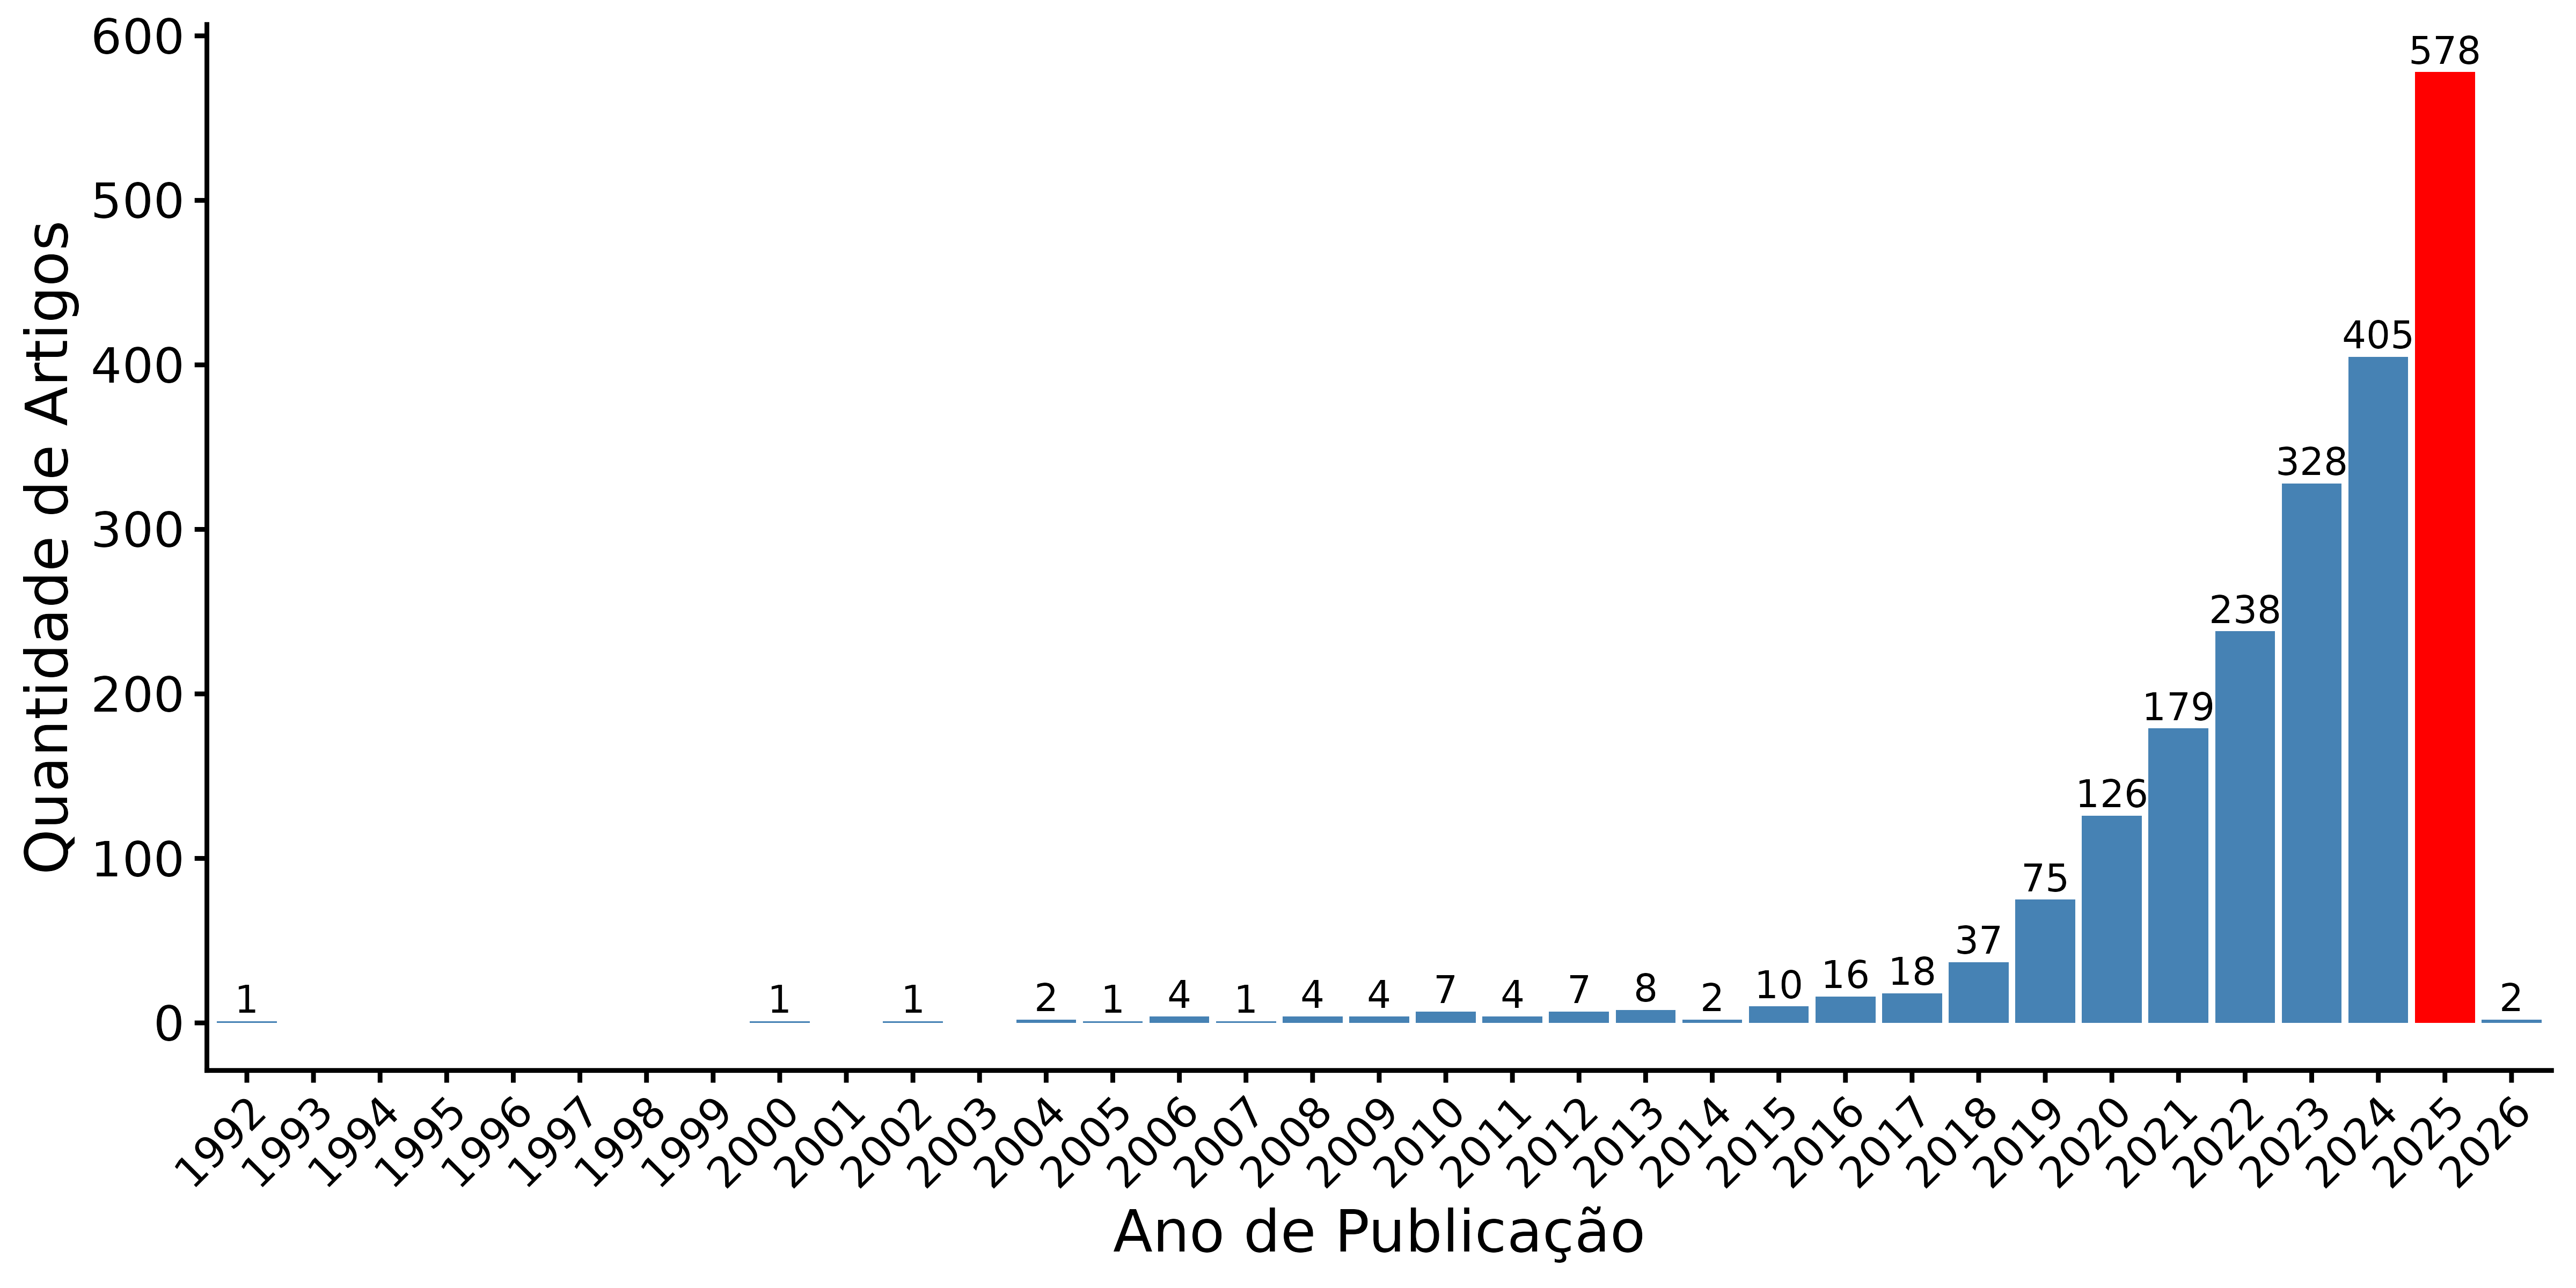
\includegraphics[width=\linewidth]{imagens/sepoc-fig2a-producao.png}
  \caption{Produção anual}
  \label{fig:producao}
\end{subfigure}\hfill
\begin{subfigure}[t]{0.49\textwidth}
  \centering
  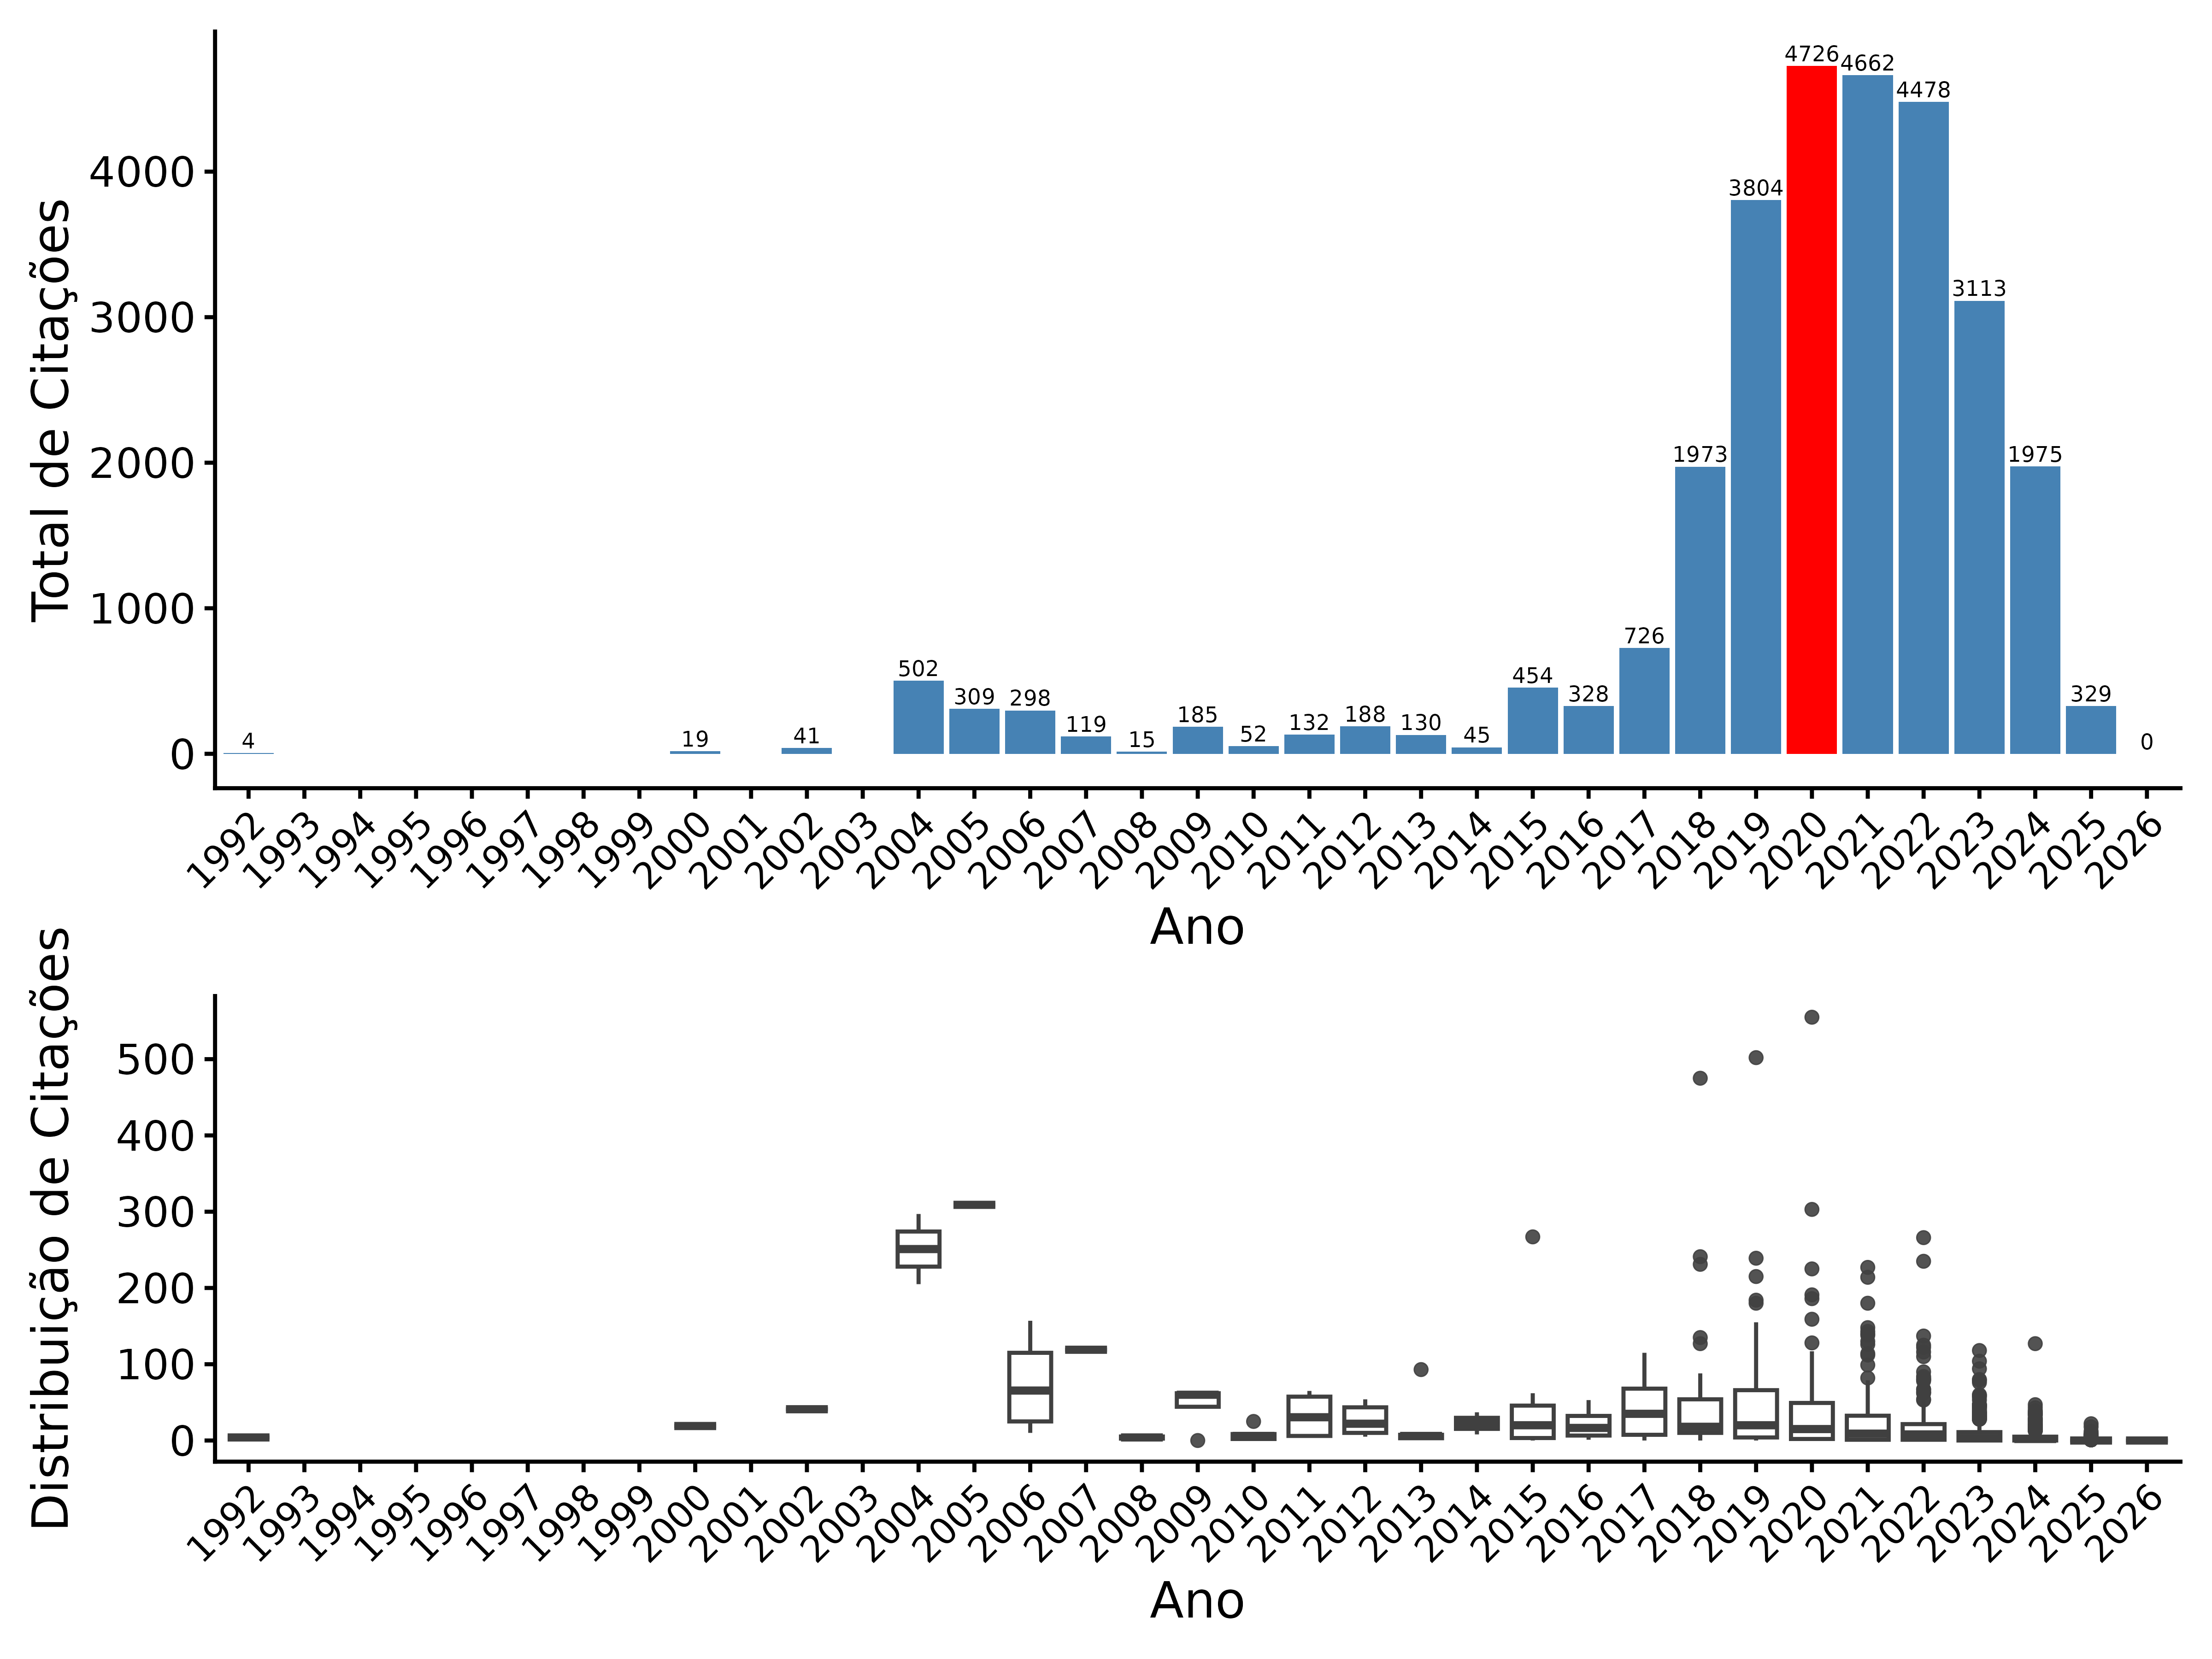
\includegraphics[width=\linewidth]{imagens/sepoc-fig2b-citacoes.png}
  \caption{Citações por ano}
  \label{fig:citacoes}
\end{subfigure}\\[2mm]
{\small Fonte: Elaborado pelos autores.}
\end{figure}

\subsection{Tecnologias e técnicas predominantes}

As categorias de DL apresentaram o crescimento mais rápido após 2018, acompanhadas por ML clássico e métodos \textit{ensemble} (Figura~\ref{fig:categorias}). Como as categorias são não excludentes, as frequências anuais podem superar o número de documentos do mesmo ano. A queda observada in 2026 é artefato do período parcial.

\textit{Machine learning} foi o termo mais frequente (1.151 ocorrências), seguido por \textit{neural network} (674), \textit{deep learning} (551), Random Forest (358), LSTM (313), \textit{ensemble} (252), CNN (223) e SVM (204) (Figura~\ref{fig:termos}). Transformers e GRU apresentaram frequências menores, compatíveis com tecnologias emergentes no período analisado. A persistência de Random Forest e SVM sugere que métodos clássicos continuam competitivos em bases de dados tabulares e em tarefas de classificação espacial, nas quais interpretabilidade, amostras moderadas e custo computacional permanecem relevantes.

\begin{figure}[!htb]
\centering
\caption{Perfil tecnológico do corpus. As contagens são frequências de ocorrência em metadados harmonizados e não representam conjuntos mutuamente exclusivos de artigos.}
\label{fig:perfil}
\begin{subfigure}[t]{0.52\textwidth}
  \centering
  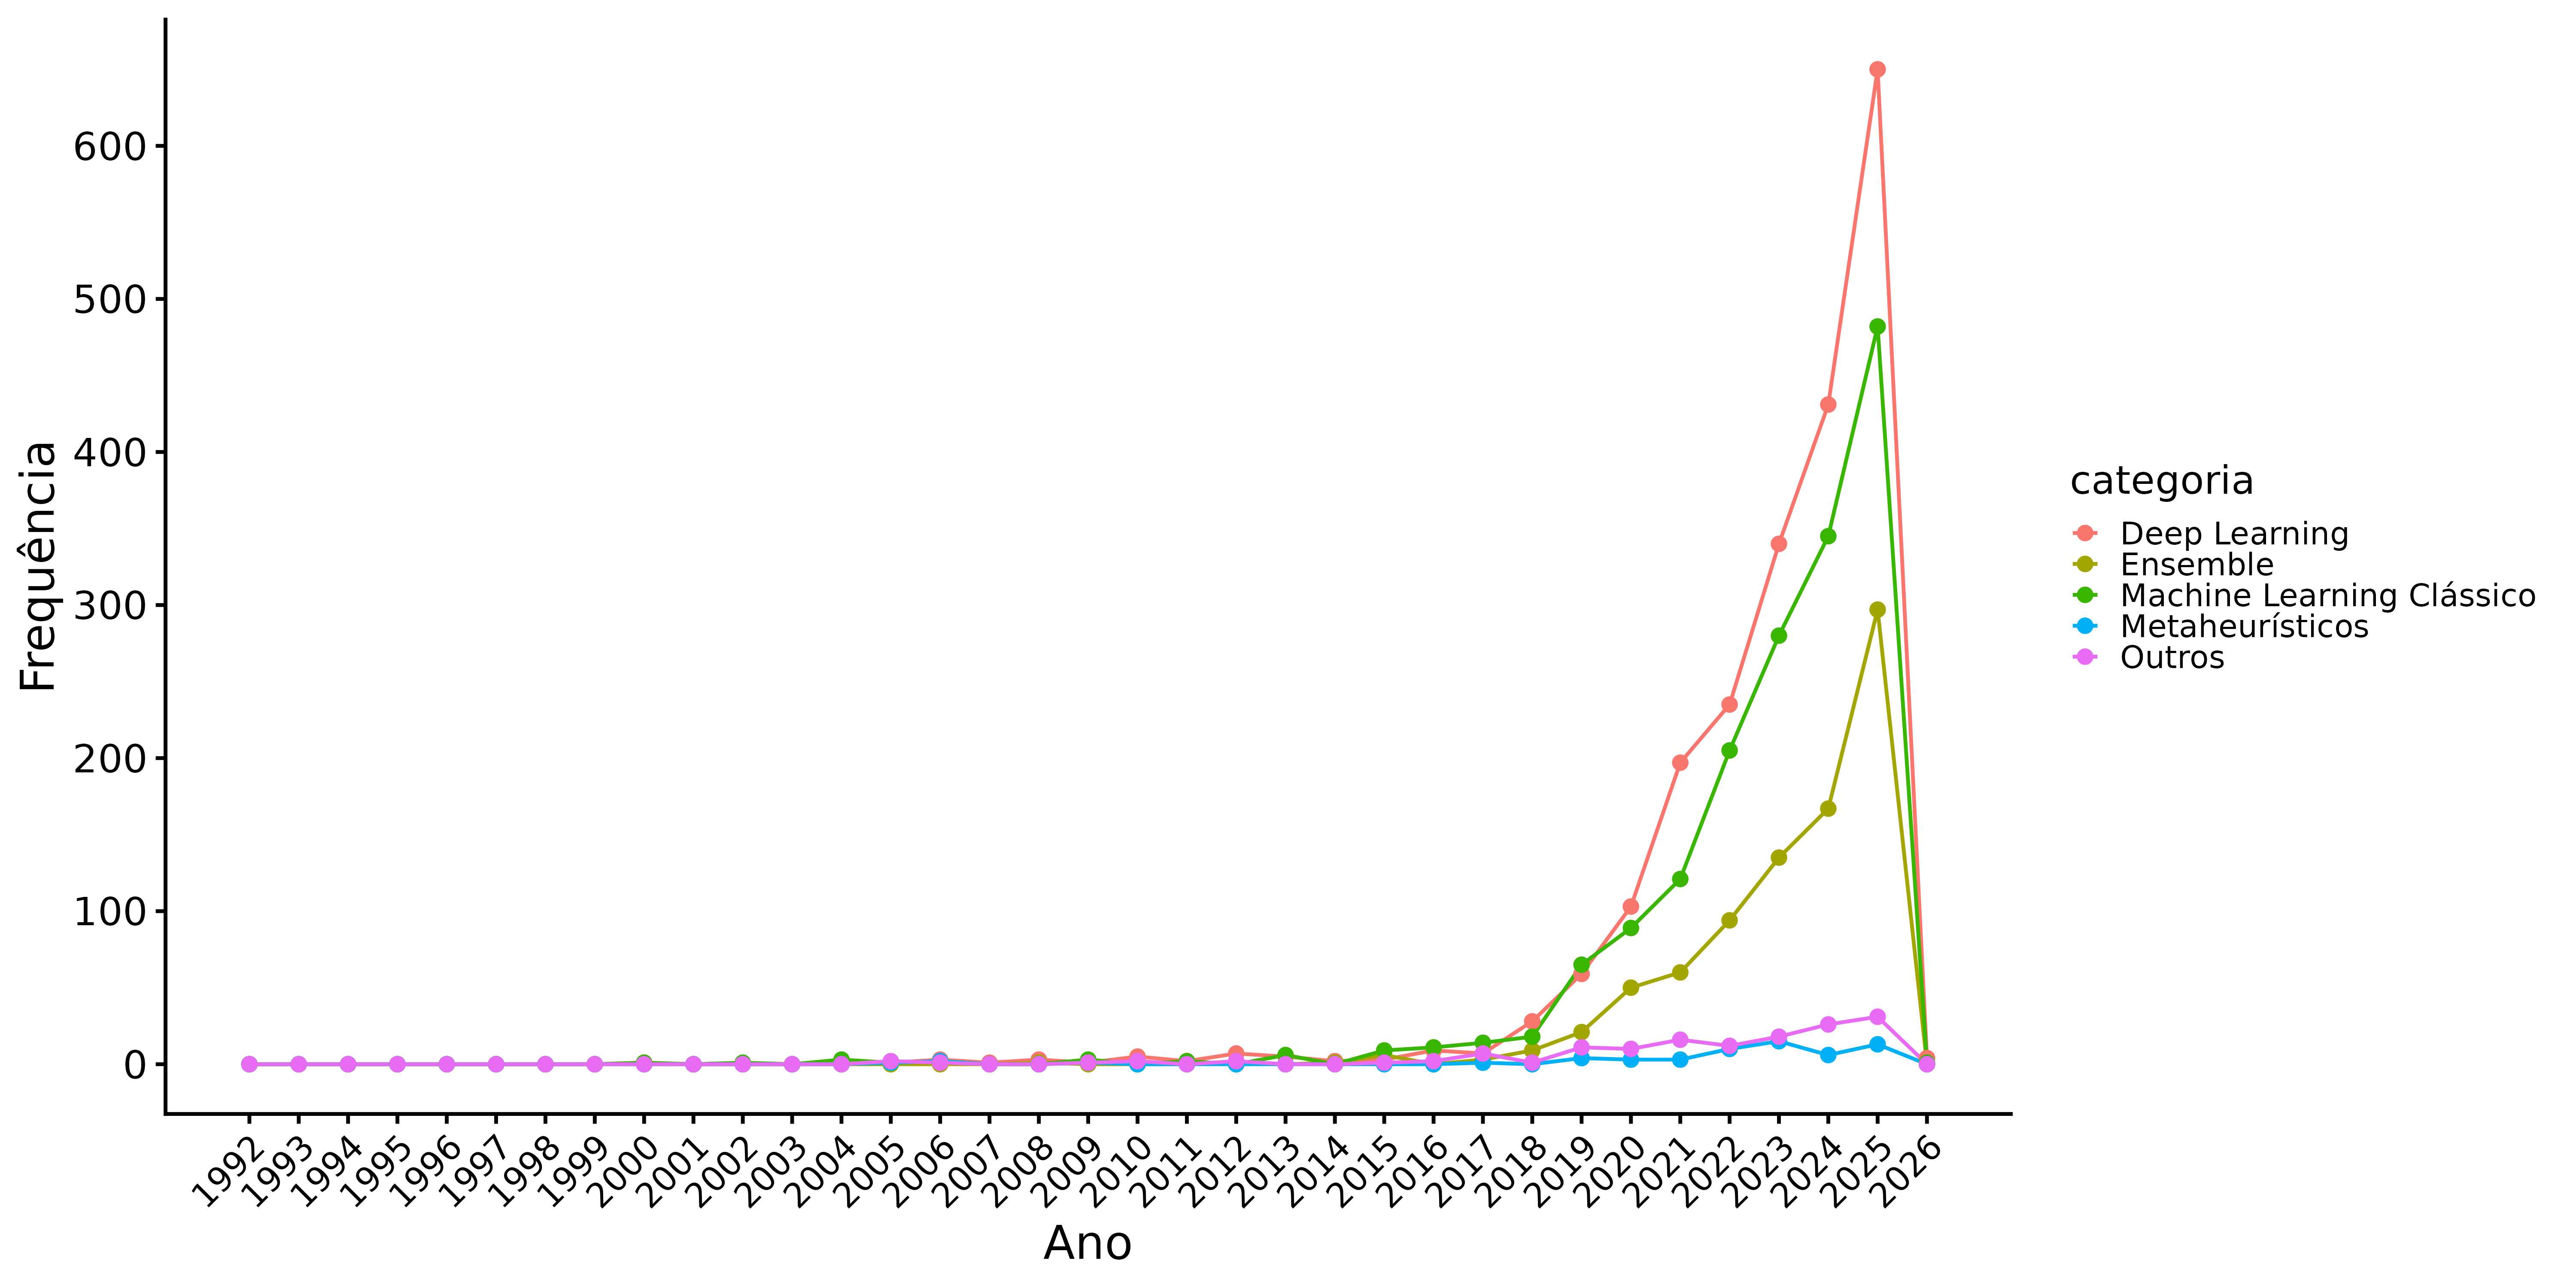
\includegraphics[width=\linewidth]{imagens/sepoc-fig3a-categorias.png}
  \caption{Categorias tecnológicas}
  \label{fig:categorias}
\end{subfigure}\hfill
\begin{subfigure}[t]{0.46\textwidth}
  \centering
  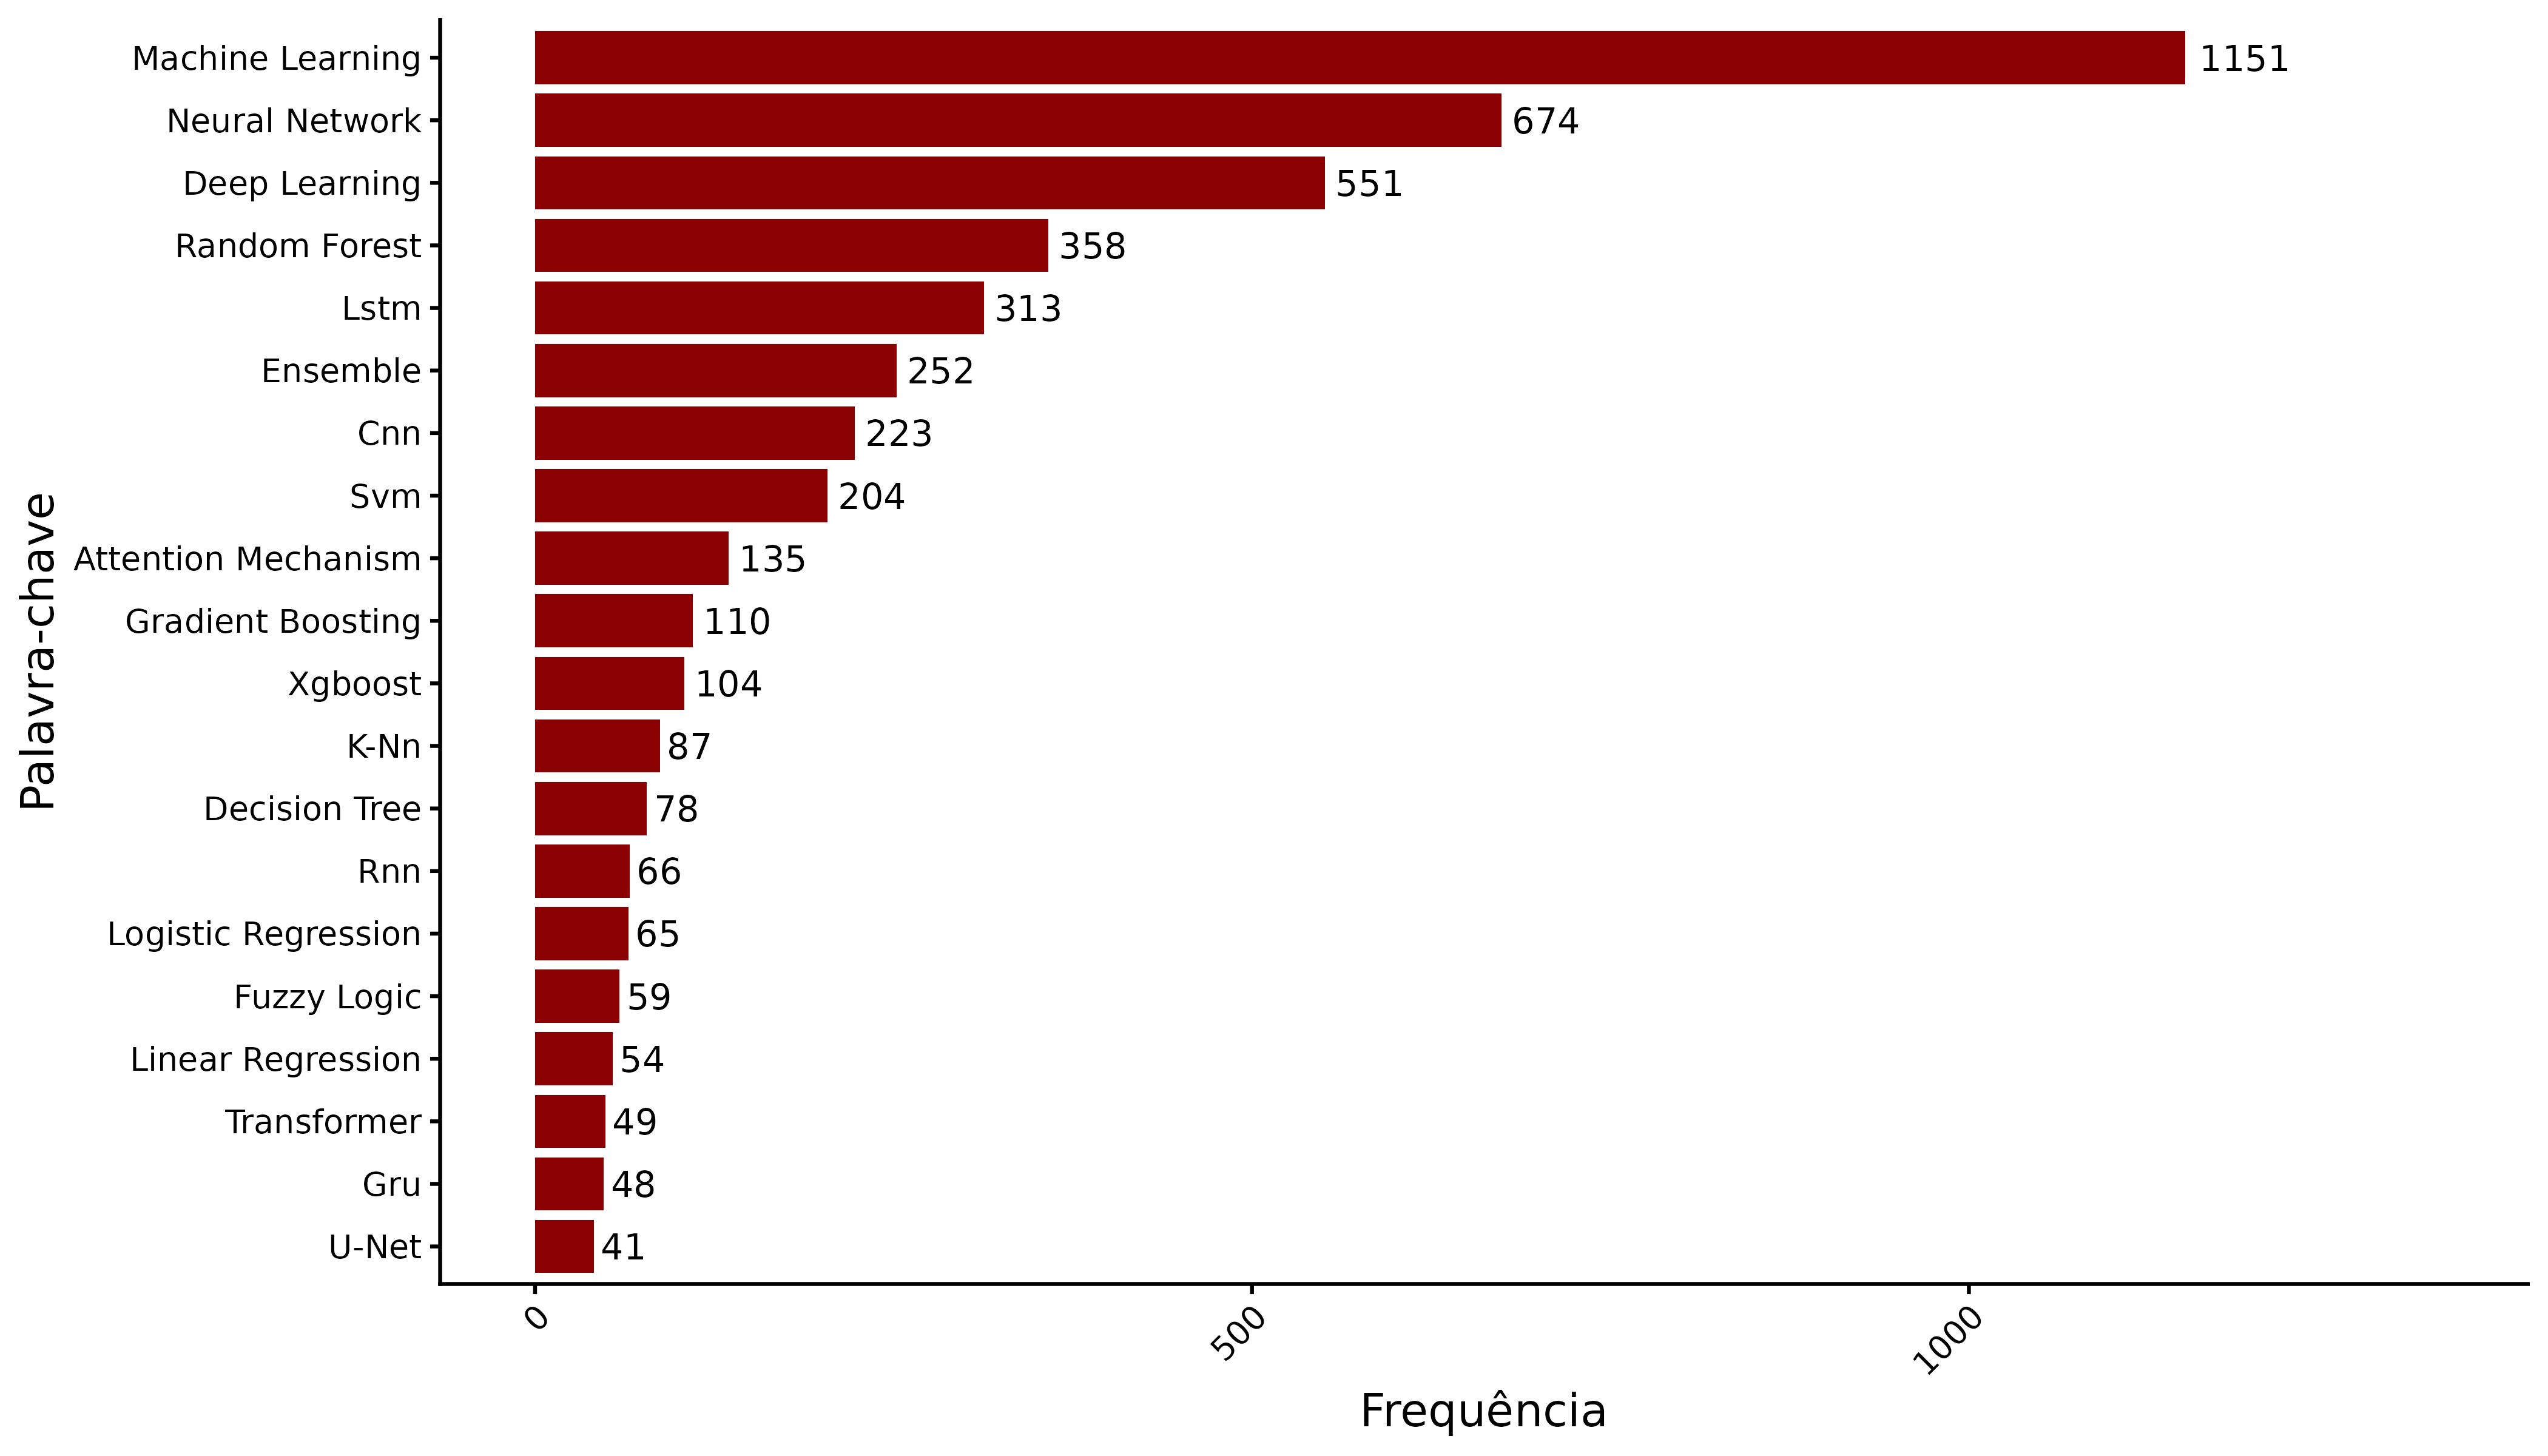
\includegraphics[width=\linewidth]{imagens/sepoc-fig3b-termos.png}
  \caption{Técnicas e termos mais frequentes}
  \label{fig:termos}
\end{subfigure}\\[2mm]
{\small Fonte: Elaborado pelos autores.}
\end{figure}

\subsection{Distribuição geográfica}

A China apresentou o maior número de publicações por afiliação (364), seguida por Estados Unidos (119) e Índia (117). Irã, Taiwan, Canadá e Vietnã também se destacaram (Figura~\ref{fig:paises}). Brasil e outros países latino-americanos não figuraram entre os 20 primeiros. Esse resultado sugere sub-representação no corpus recuperado, mas não comprova ausência de estudos, pois depende da estratégia de busca, da cobertura das bases, do idioma e do método de contagem de afiliações.

\begin{figure}[!htb]
\centering
\caption{Países com maior número de publicações segundo os metadados de afiliação. A unidade geográfica não deve ser confundida com o local de aplicação empírica do estudo.}
\label{fig:paises}
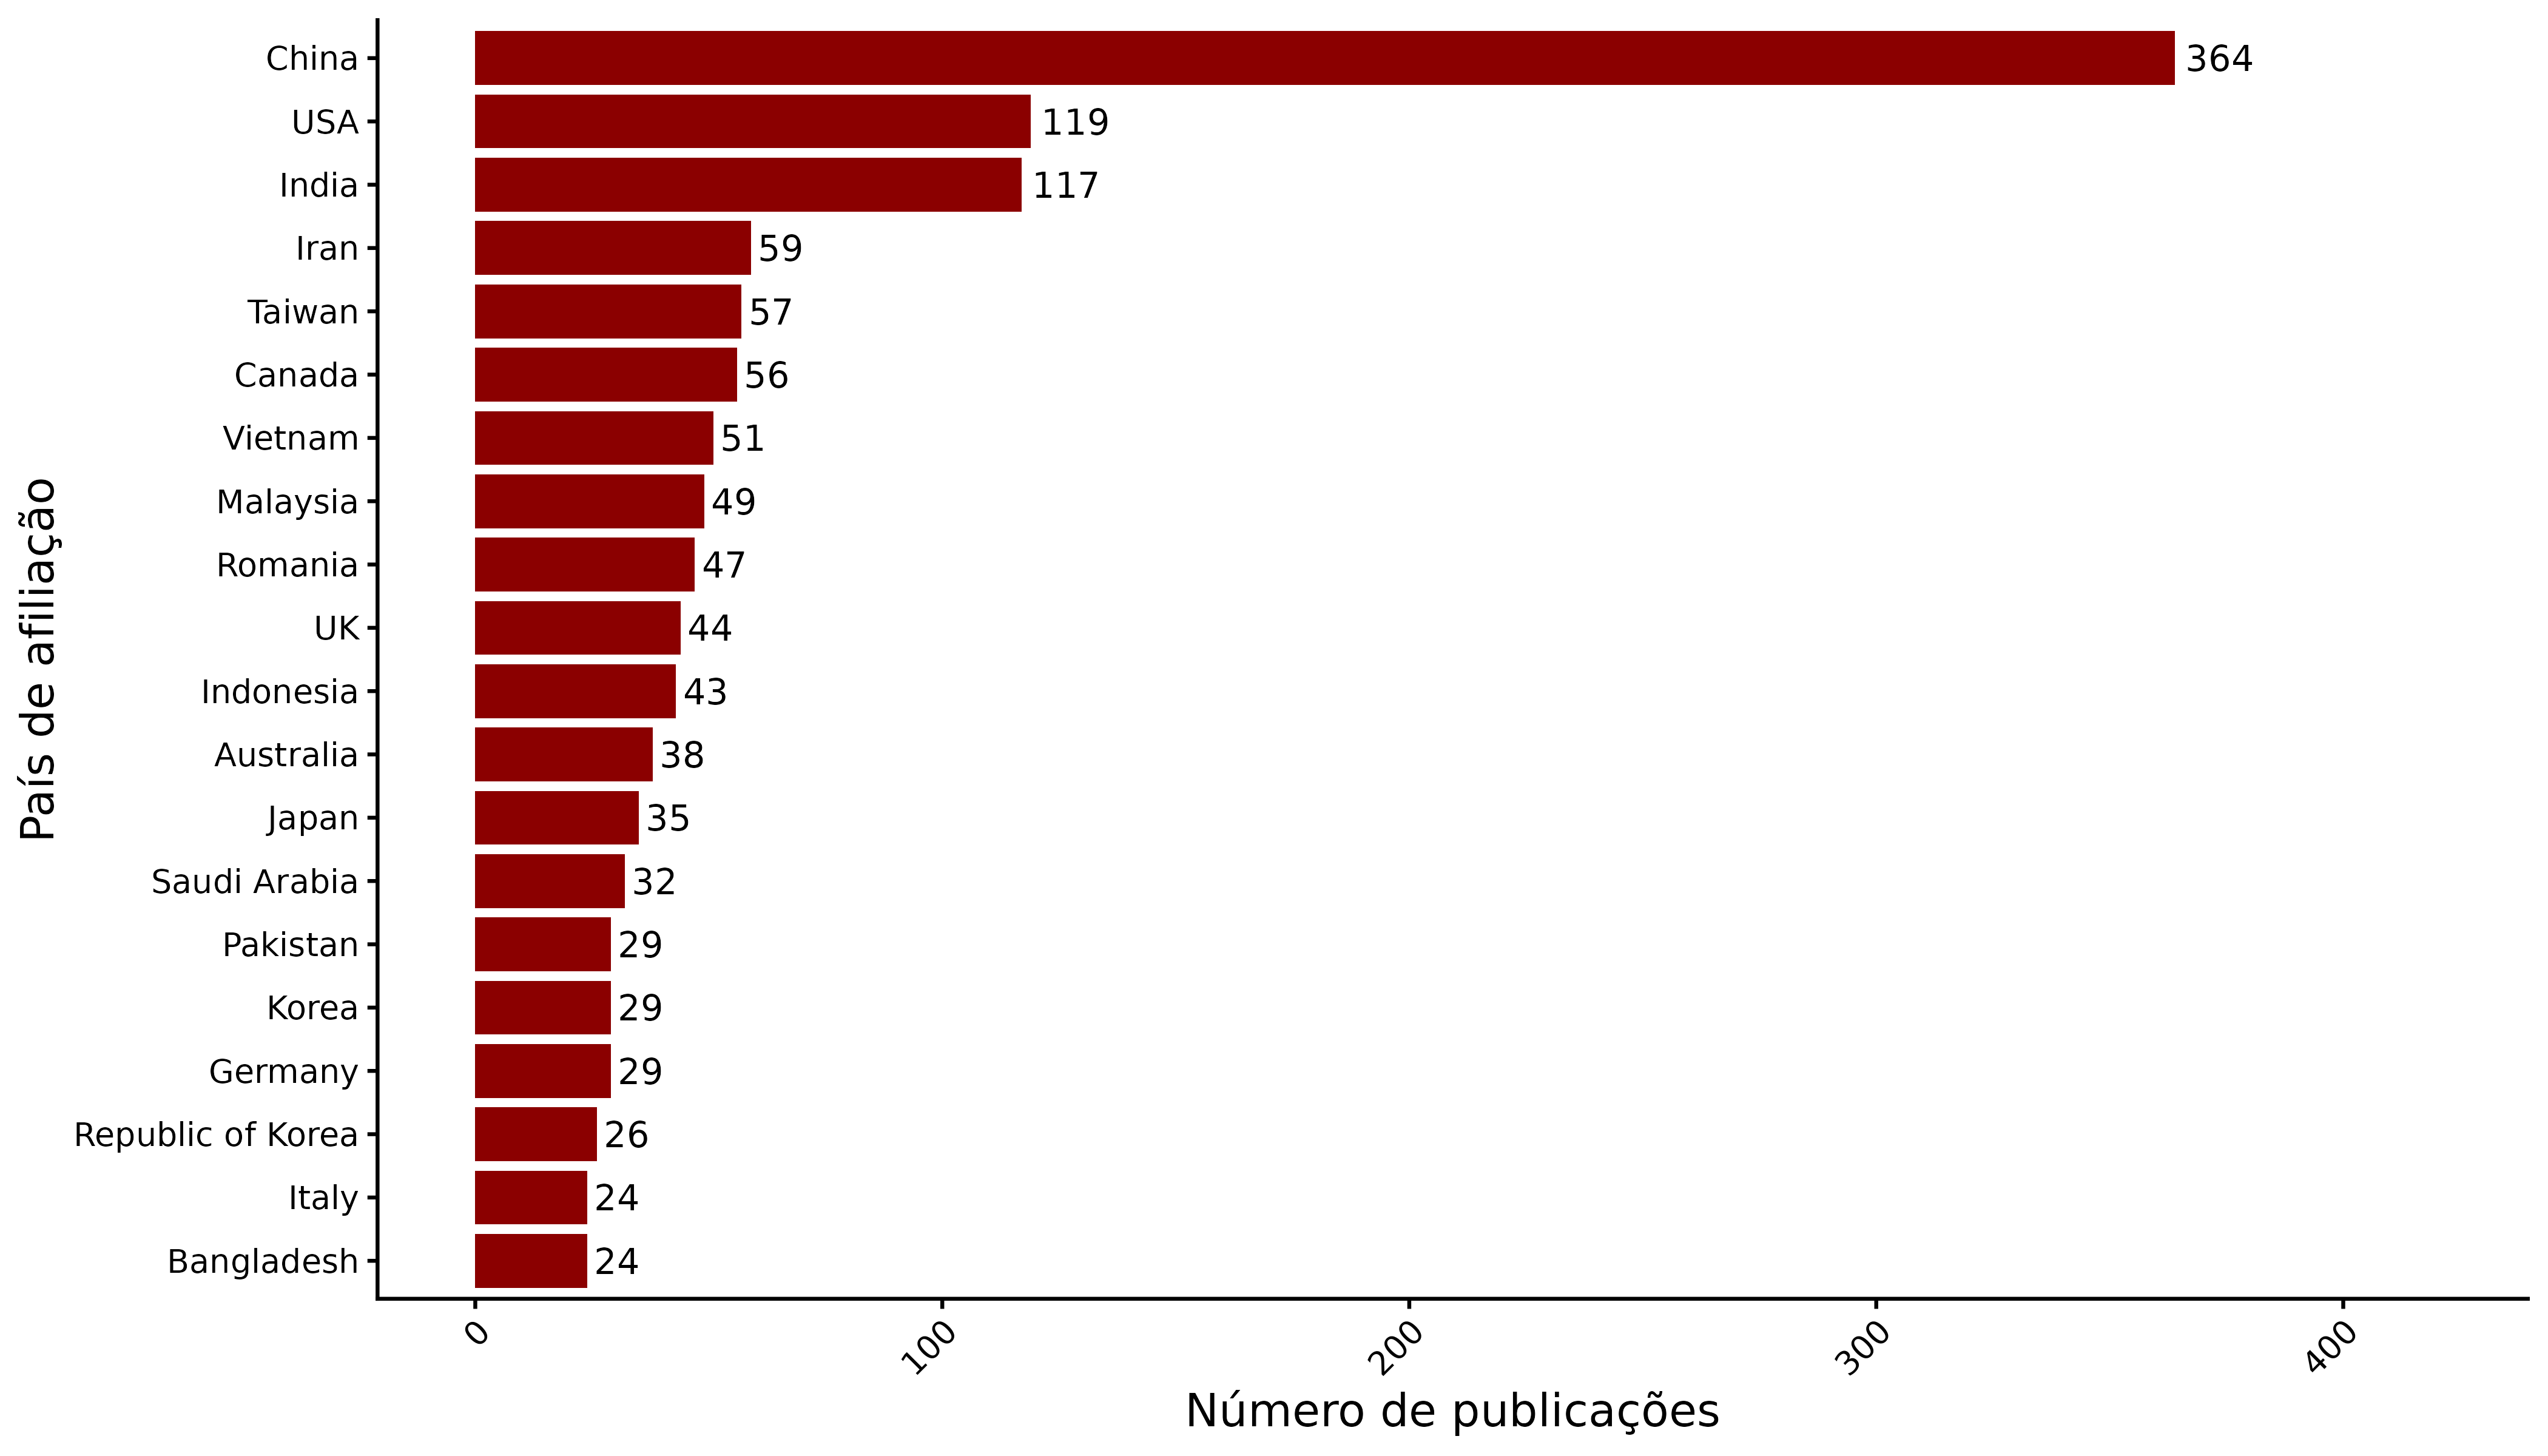
\includegraphics[width=0.75\textwidth]{imagens/sepoc-fig4-paises.png}\\[2mm]
{\small Fonte: Elaborado pelos autores.}
\end{figure}

\subsection{Síntese dos artigos de maior prioridade}

Os 13 artigos do Núcleo A foram publicados predominantemente entre 2018 e 2022 e apresentaram média de 283 citações na base consolidada. A Tabela~\ref{tab:nucleoA} evidencia que o estrato não é composto apenas por previsão temporal, predominam o mapeamento de suscetibilidade, a classificação espacial e a integração com sensoriamento remoto. Essa composição explica a coexistência de métricas hidrológicas, como NSE e R$^2$, com métricas de classificação, como AUC, acurácia, sensibilidade e especificidade.

{\small
\renewcommand{\arraystretch}{1.2}
\begin{longtable}{@{}p{2.7cm}p{2.6cm}p{3.1cm}p{5.6cm}@{}}
\caption{Síntese funcional dos 13 artigos do Núcleo A. Valores de desempenho não são comparados porque tarefas, dados, escalas e desenhos de validação diferem entre estudos.}\label{tab:nucleoA}\\
\toprule
\textbf{Estudo} & \textbf{Tarefa principal} & \textbf{Método} & \textbf{Contribuição científica central}\\
\midrule
\endfirsthead
\toprule
\textbf{Estudo} & \textbf{Tarefa principal} & \textbf{Método} & \textbf{Contribuição científica central}\\
\midrule
\endhead
\midrule
\multicolumn{4}{r}{\footnotesize\textit{continua na próxima página}}\\
\endfoot
\bottomrule
\multicolumn{4}{@{}l}{\footnotesize Fonte: Elaborado pelos autores.}\\
\endlastfoot
\citeonline{xiang2020} & Previsão chuva--vazão & LSTM \textit{sequence-to-sequence} & Previsão em múltiplos passos e representação de dependências temporais.\\
\citeonline{tyralis2019} & Revisão metodológica & Random Forest e variantes & Sistematização do uso de florestas aleatórias em recursos hídricos e importância de variáveis.\\
\citeonline{hu2018} & Simulação chuva--vazão & LSTM & Aplicação de memória recorrente à dinâmica hidrológica e aos picos de vazão.\\
\citeonline{janizadeh2019} & Suscetibilidade a enxurradas & ADT, FT, KLR, MLP e QDA & Comparação de classificadores sobre fatores geoambientais.\\
\citeonline{dodangeh2020} & Suscetibilidade & GAM, MARS, BRT e reamostragem & Tratamento do desbalanceamento entre ocorrências e não ocorrências.\\
\citeonline{rafieisardooi2021} & Risco urbano & ML e TOPSIS & Integração entre perigo físico e vulnerabilidade socioeconômica.\\
\citeonline{zhao2019} & Suscetibilidade urbana & WELLSVM semissupervisionado & Aproveitamento de dados não rotulados em inventários incompletos.\\
\citeonline{fang2021} & Suscetibilidade & LSTM & Uso de arquitetura recorrente em padrões espaciais de condicionantes.\\
\citeonline{costache2020} & Suscetibilidade a enxurradas & KNN, AHP e análise multicritério & Integração entre ML, sensoriamento remoto, SIG e decisão multicritério.\\
\citeonline{shahabi2020} & Detecção e suscetibilidade & Sentinel-1 e \textit{ensemble} Bagging--KNN & Combinação de velocidade da Terra com classificadores \textit{ensemble}.\\
\citeonline{arora2021} & Suscetibilidade & ANFIS com GA, DE e PSO & Otimização metaheurística de modelos neurodifusos.\\
\citeonline{wu2020} & Revisão de previsão & Previsão probabilística \textit{ensemble} & Ênfase em incerteza, assimilação de dados e uso operacional.\\
\citeonline{saha2021} & Suscetibilidade & Hyperpipes, SVR e \textit{ensemble} HP--SVR & Combinação de algoritmos com perfis complementares de classificação.\\
\end{longtable}
}

% ---------------------------------------------------------------------
\section{Discussão}
\label{sec:art-discussao}

\subsection{Crescimento bibliométrico não equivale à maturidade operacional}

O aumento de publicações revela forte mobilização científica, mas não demonstra, isoladamente, ganho em termos de generalização, robustez ou utilidade operacional. Parte do crescimento decorre da expansão dos dados de sensoriamento remoto, das reanálises meteorológicas, dos sensores de baixo custo e da infraestrutura computacional. O avanço mais relevante ocorre quando modelos são avaliados fora da amostra, em bacias, períodos e extremos não utilizados no treinamento. O sistema global analisado por \citeonline{nearing2024} empregou validação espacial e temporal explícita e comparação com um sistema operacional de referência, oferecendo um padrão mais exigente do que o de divisões aleatórias de treino e teste.

\subsection{A tarefa científica deve preceder a escolha do algoritmo}

A principal fragilidade conceitual do corpus é o uso indiscriminado de ``previsão de inundação'' para tarefas distintas. A previsão hidrológica estima estados futuros e requer horizonte de antecedência, persistência, erro de pico, NSE, KGE, viés e calibração probabilística. Mapeamento de suscetibilidade estima a propensão espacial e costuma empregar AUC, sensibilidade, especificidade e acurácia. A detecção de inundação segmenta áreas afetadas em imagens e requer métricas como IoU e F1. Avaliação de risco combina perigo, exposição e vulnerabilidade, não podendo ser reduzida à acurácia de um classificador.

Consequentemente, valores elevados de AUC em um mapa de suscetibilidade não podem ser interpretados como evidência de capacidade de alerta em tempo real; da mesma forma, um bom NSE médio não garante reprodução dos extremos que interessam à defesa civil. Comparações futuras devem ser estratificadas por tarefa, escala, horizonte, fonte de dados e protocolo de validação.

\subsection{Validação, dependência espacial e incerteza}

Dados hidrológicos e geoespaciais apresentam autocorrelação temporal e espacial. Divisões aleatórias podem colocar observações muito semelhantes nos conjuntos de treino e teste, produzindo estimativas otimistas de desempenho. A validação bloqueada no espaço, no tempo e por evento, bem como testes em bacias não observadas, são necessários para avaliar a transferência real \cite{roberts2017}. Para aplicações operacionais, recomenda-se comparar a IA com referências simples e modelos físicos, reportar o desempenho por horizonte e por magnitude do evento, quantificar a incerteza e avaliar a calibração probabilística.

Modelos híbridos e guiados por conhecimento oferecem uma direção promissora, pois podem combinar flexibilidade estatística com restrições de balanço hídrico, de conectividade de drenagem e de coerência física \cite{nearing2021}. A interpretabilidade também deve ser tratada como requisito de segurança e de diagnóstico, e não apenas como recurso de visualização posterior.

\subsection{Lacuna costeira, desigualdade de dados e aplicabilidade regional}

A baixa representação latino-americana e a ausência de contextos costeiros brasileiros no Núcleo A são relevantes, mas precisam ser interpretadas com cautela. A própria expressão de busca privilegia termos genéricos e urbanos e não inclui explicitamente vocabulário de inundação costeira ou composta. Assim, parte da lacuna observada é substantiva e outra pode ser decorrente do desenho da busca.

Em municípios costeiros, modelos devem integrar precipitação, nível do rio, maré, sobreelevação meteorológica, ondas, impermeabilização e capacidade da drenagem. A análise isolada desses componentes pode subestimar eventos compostos \cite{wahl2015}. Para cidades médias e regiões com monitoramento limitado, a agenda mais promissora combina sensores locais, radar meteorológico, produtos de satélite, reanálises, modelos hidrodinâmicos simplificados e IA com transferência entre bacias. Dados abertos e protocolos comuns de validação são fundamentais para reduzir a desigualdade entre regiões bem monitoradas e áreas altamente vulneráveis.

\subsection{Agenda de pesquisa}

Os resultados sustentam cinco prioridades: (i) ampliar a estratégia de busca com vocabulário costeiro, composto e operacional; (ii) separar análises por tarefa científica; (iii) adotar validação espaço-temporal e por eventos extremos; (iv) combinar previsão pontual com incerteza, interpretabilidade e coerência física, e; (v) disponibilizar exportações, dicionários de palavras-chave, código de deduplicação e cálculo do escore. A tendência de adoção de Transformers e arquiteturas mais profundas é relevante. Entretanto, a maior complexidade dos modelos deve ser acompanhada por protocolos rigorosos de validação. Quando informações do período, local ou evento usado para avaliação também influenciam o treinamento, a potencial ocorrência de \textit{data leakage} passa a ser aumentada, produzindo assim estimativas artificialmente elevadas de desempenho e pouca capacidade de generalização do modelo e detecção de novas enchentes.

% ---------------------------------------------------------------------
\section{Limitações}
\label{sec:art-limitacoes}

Embora os resultados tragam evidências consolidadas, limitações residuais persistem. Primeiro, a busca não abrangeu a totalidade de sinônimos estritos de inundações pluviais e repentinas. Segundo, a exclusão de bases complementares como Web of Science restringe marginalmente a captação de dinâmicas regionais periféricas. Terceiro, o viés de indexação incompleta inviabiliza o uso pleno de dados de 2026. Quarto, as contagens por país refletem vínculos institucionais e não capturam necessariamente a localização empírica da bacia hidrográfica avaliada. Por fim, a dependência inerente a termos indexados pode omitir nuances que escapam às convenções formais de palavras-chave.

% ---------------------------------------------------------------------
\section{Conclusão}
\label{sec:art-conclusao}

A literatura sobre IA aplicada a inundações expandiu-se rapidamente, com concentração de publicações após 2018 e crescimento de DL, LSTM, CNN e métodos \textit{ensemble}. Random Forest, SVM e outras abordagens clássicas permanecem relevantes, especialmente no mapeamento espacial. China, Estados Unidos e Índia lideraram a produção por afiliação, enquanto a América Latina apareceu de forma limitada no recorte analisado.

A principal conclusão científica é que o campo não deve ser avaliado como um bloco homogêneo. Previsão temporal, detecção, suscetibilidade e risco associam-se a perguntas diferentes, utilizam métricas distintas e exigem protocolos específicos de validação. A próxima etapa de maturidade depende de generalização espaço-temporal, avaliação de extremos, quantificação de incerteza, integração com processos físicos e reprodutibilidade aberta. Para municípios costeiros do Sul do Brasil, estudos futuros devem considerar explicitamente inundações compostas e integrar observações locais, sensoriamento remoto, maré, chuva, drenagem e modelos híbridos orientados à decisão e ao alerta precoce.

\section{Trabalhos relacionados}
\label{sec:trabalhos-relacionados}
% =====================================================================
% Revisão bibliográfica -- texto do projeto de dissertação
% =====================================================================

O uso de técnicas de inteligência artificial na previsão de eventos hidrológicos tem ganhado destaque nos últimos anos, diante das limitações dos modelos estatísticos tradicionais e da necessidade de soluções mais eficientes frente às mudanças climáticas. Entre essas técnicas, as Redes Neurais Artificiais (RNAs), especialmente as redes profundas como LSTM e as redes multicamadas do tipo perceptron, têm se mostrado promissoras na modelagem de dados ambientais com comportamento não linear.

\citeonline{oliveira2013} aplicaram RNAs à previsão de vazões em rios urbanos, evidenciando ganhos expressivos de precisão em relação a métodos tradicionais baseados em regressão linear. Em estudo regional, \citeonline{soares2015} implementaram redes neurais para previsão de cheias no Rio Itajaí-Açu, em Santa Catarina, com resultados que demonstram a viabilidade dessas abordagens em cenários locais.

\citeonline{mosavi2018} realizaram uma análise comparativa abrangente entre diversos modelos de aprendizado de máquina aplicados à previsão de enchentes, concluindo que as redes neurais profundas superam algoritmos mais simples, especialmente em ambientes com alta variabilidade de dados e múltiplas variáveis de entrada.

No contexto urbano brasileiro, \citeonline{valle2021} utilizou RNAs para prever o número de ruas alagadas em Curitiba, obtendo coeficientes de determinação superiores a 0,95. \citeonline{estrada2021} aplicou redes neurais à previsão da demanda hídrica em Joinville (SC), destacando o potencial dessas técnicas para auxiliar no planejamento e na gestão de recursos hídricos.

\citeonline{magro2022} também demonstrou a eficiência das RNAs na previsão de profundidade de alagamentos em áreas urbanas da cidade de Lages (SC), com enfoque na construção de um sistema de alerta. Seus resultados indicaram que modelos com múltiplas saídas apresentaram melhor desempenho na redução de erros e aumento da confiabilidade preditiva.

Apesar dos avanços, ainda existem lacunas significativas. A maioria dos estudos concentra-se na previsão de variáveis hidrológicas específicas, como vazão ou nível de rios, mas poucos integram variáveis socioeconômicas e dados geoespaciais ao processo de modelagem. A integração desses elementos é essencial para avaliar não apenas o risco físico, mas também a vulnerabilidade social e a capacidade de resposta das comunidades afetadas.

Dessa forma, esta pesquisa se propõe a atuar nessa lacuna, integrando dados ambientais e sociais por meio de técnicas de inteligência artificial, com foco nas comunidades costeiras de Santa Catarina. A revisão da literatura indica que há um terreno fértil para inovação metodológica e aplicação prática, o que reforça a relevância científica e social da proposta.

\begin{table}[!htb]
\caption{Resumo dos principais trabalhos revisados}
\label{tab:revisao}
\centering
\small
\renewcommand{\arraystretch}{1.2}
\begin{tabular}{@{}p{3.4cm}p{3.6cm}p{\dimexpr\textwidth-7cm-4\tabcolsep\relax}@{}}
\toprule
\textbf{Autor(es)} & \textbf{Contexto} & \textbf{Contribuição}\\
\midrule
\citeonline{oliveira2013} & Rios urbanos (Brasil) & Previsão de vazão com RNAs, mais precisas que modelos estatísticos tradicionais.\\
\citeonline{soares2015} & Bacia do Rio Itajaí-Açu & Aplicação regional de IA para previsão de cheias com bons resultados.\\
\citeonline{mosavi2018} & Revisão internacional & Avaliação de diversos algoritmos de IA, com destaque para redes neurais profundas.\\
\citeonline{valle2021} & Curitiba/PR & Previsão de alagamentos urbanos com RNAs, alta precisão preditiva.\\
\citeonline{estrada2021} & Joinville/SC & Demanda hídrica urbana com RNAs, reforçando aplicabilidade local.\\
\citeonline{magro2022} & Lages/SC & Alerta de alagamentos com RNAs multivariadas, foco em sistema preventivo.\\
\bottomrule
\end{tabular}\\[1mm]
{\small Fonte: Elaborado pela autora.}
\end{table}

\chapter{Desenvolvimento}
\label{chp:desenvolvimento}
\pendente{Capítulo a escrever: base de dados integrada, pré-processamento, definição de variáveis, arquitetura e treinamento dos modelos.}

\chapter{Resultados}
\label{chp:resultados}
\pendente{Capítulo a escrever: resultados, validação e comparação entre modelos.}

\chapter{Conclusão}
\label{chp:conclusao}
% =====================================================================
% Considerações finais -- texto do projeto de dissertação
% (substituir pelas conclusões da dissertação quando os resultados
% estiverem prontos)
% =====================================================================

Este projeto busca oferecer uma solução tecnológica robusta, baseada em inteligência artificial, para a antecipação de enchentes em comunidades costeiras catarinenses. Ao integrar variáveis ambientais, hidrológicas e socioeconômicas, espera-se contribuir com conhecimento científico relevante e apoio técnico à tomada de decisões em políticas públicas de gestão de risco. A abordagem proposta é inovadora no contexto regional e se alinha aos desafios contemporâneos impostos pelas mudanças climáticas.




% ---
% Finaliza a parte no bookmark do PDF, para que se inicie o bookmark na raiz
% ---
\bookmarksetup{startatroot}% 
% ---

% ----------------------------------------------------------
% ELEMENTOS PÓS-TEXTUAIS
% ----------------------------------------------------------
\postextual

% ----------------------------------------------------------
% Referências bibliográficas
% ----------------------------------------------------------
% Itens da lista de referências dos textos originais que não são citados no texto:
\nocite{islam2025,ana2021}
\bibliography{references}
% Bibliography
\printglossary
% ---------------------------------------------------------------------
% GLOSSÁRIO
% ---------------------------------------------------------------------

% Arquivo que contém as definições que vão aparecer no glossário
%\input{tex/glossario}
% Comando para incluir todas as definições do arquivo glossario.tex
%\glsaddall
% Impressão do glossário
%\printglossaries

% ----------------------------------------------------------
% Apêndices
% ----------------------------------------------------------

% ---
% Inicia os apêndices
% ---
% Apêndices e anexos do modelo (textos de exemplo), desativados:
% \begin{apendicesenv}

%     \chapter{Apenas para Exemplo}
%     \label{Apendice_A}
% Aqui você colocaria o texto que iria aparecer no Apêndice. Caso não precise é só comentar essa parte.

    
%   %  \label{chapter:documento-basico}
%   %  \definecolor{gray}{rgb}{0.4,0.4,0.4}
\definecolor{darkblue}{rgb}{0.0,0.0,0.6}
\definecolor{cyan}{rgb}{0.0,0.6,0.6}
\definecolor{maroon}{rgb}{0.5,0,0}
\definecolor{darkgreen}{rgb}{0,0.5,0}


\lstdefinelanguage{myLatex}
{
    keywords={\titulo},
    alsoletter={-},
    sensitive=false,
    morecomment=[l]{\%},
    morecomment=[s]{/*}{*/},
    morestring=[b]",
    morestring=[b]',
    keywordstyle=\bfseries\color{blue},
    commentstyle=\itshape\color{darkgreen},
    morekeywords={documentclass, titulo, autor, data, orientador, coorientador, curso, textoresumo, incluifichacatalografica, textodedicatoria*, textoagradecimentos*, textoepigrafe*, incluilistadefiguras, incluilistadetabelas, incluilistadequadros, incluilistadealgoritmos, incluilistadecodigos, incluilistadesiglas, incluilistadesimbolos, textual, chapter, postextual, begin, bibliography, end}, 
alsoletter={*, \{, \}, \[, \]},
 morekeywords=[2]{\{, \}, \[, \]},
 keywordstyle=[2]\bfseries\color{blue},
 moredelim=[s][\color{maroon}]{\{}{\}},
    moredelim=[s][\itshape\color{maroon}]{\[}{\]},
}

%\lstdefinelanguage{TeX}
%{
%moredelim=*[s][\color{maroon}]{\{}{\}}
%otherkeywords={\{, \}, \[, \], \\}
%  morestring=[b]",
%  moredelim=[s][\bfseries\color{maroon}]{<}{\ },
%  moredelim=[s][\bfseries\color{maroon}]{</}{>},
%  moredelim=[l][\bfseries\color{maroon}]{/>},
%  moredelim=[l][\bfseries\color{maroon}]{>},
%  commentstyle=\color{darkgreen},
%  stringstyle=\color{blue},
%  identifierstyle=\color{red},
%  keywordstyle=\bfseries\color{maroon}
%moredelim=[l][\bfseries\color{maroon}]{>},
%commentstyle=\color{darkgreen},
%  stringstyle=\color{blue},
%  identifierstyle=\color{red}, moredelim=[l][\bfseries\color{maroon}]{\{},
%  keywordstyle=\bfseries\color{maroon}
%}

%\lstset{language={[LaTeX]TeX},
%texcsstyle=*\bfseries\color{blue},
%keywordstyle=\bfseries\color{blue},
%commentstyle=\color{darkgreen},
%morecomment=[s][\color{red}]{\{}{\}},
%otherkeywords={$, \{, \}, \[, \]}
%}

%\begin{codigo}[caption={Exemplo de um documento básico}, label={codigo:documento-basico}, language={[LaTeX]TeX},  breaklines=true,morekeywords={titulo, autor, data, orientador, coorientador, curso, textoresumo, incluifichacatalografica, textodedicatoria*, textoagradecimentos*, textoepigrafe*, incluilistadefiguras, incluilistadetabelas, incluilistadequadros, incluilistadealgoritmos, incluilistadecodigos, incluilistadesiglas, incluilistadesimbolos, {\backslash}textual, chapter, postextual}, alsoletter={{\backslash},*},morecomment=[s][\color{red}]{\{}{\}}]
\begin{codigo}[caption={Exemplo de um documento básico}, label={codigo:documento-basico}, language={myLatex},  breaklines=true]
% Documento utilizando a classe icmc
% Opções: 
%   Qualificação          = qualificacao 
%   Curso                 = doutorado/mestrado
%   Situação do trabalho  = pre-defesa/pos-defesa (exceto para qualificação)
%   Versão para impressão = impressao
\ documentclass[doutorado, pos-defesa]{packages/icmc}

% Título do trabalho em Português
\tituloPT{Título da Monografia}

% Título do trabalho em Inglês
\tituloEN{Título da Monografia}

% Nome do autor
\autor[Abreviação]{Nome completo do autor}

% Gênero do autor (M ou F)
\genero{M}

% Data do depósito
\data{18}{12}{2012}

% Nome do Orientador
\orientador[Orientador]{Titulação do orientador}{Nome completo do Orientador}

% Nome do Coorientador (caso não exista basta remover)
\coorientador[Coorientador]{Titulação do coorientador}{Nome completo do Coorientador}
% Se coorientadora troque Coorientador: por Coorientadora dentro do colchetes

% Sigla do programa de Pós-graduação (CCMC, MAT, PIPGES, PROFMAT, MECAI)
\curso{CCMC}
% O valor entre colchetes é opcional para este programa

% Idioma principal do texto (EN ou PT)
\idioma{PT}

% Resumo
\textoresumo[Idioma]{
Texto do resumo do trabalho.
}{Lista de palavras-chave separada por virgulas}

% ----------------------------------------------------------
% ELEMENTOS PRÉ-TEXTUAIS
% ----------------------------------------------------------

% Inserir a ficha catalográfica
%\incluifichacatalografica{tex/ficha-catalografica.pdf}

% Incluí o texto da Dedicatória
\textodedicatoria*{tex/pre-textual/dedicatoria}

% Incluí o texto dos Agradecimentos
\textoagradecimentos*{tex/pre-textual/agradecimentos}

% Incluí o texto da Epígrafe
\textoepigrafe*{tex/pre-textual/epigrafe}

% Inclui a lista de figuras
\incluilistadefiguras

% Inclui a lista de tabelas
\incluilistadetabelas

% Inclui a lista de quadros
\incluilistadequadros

% Inclui a lista de algoritmos
\incluilistadealgoritmos

% Inclui a lista de códigos
\incluilistadecodigos

% Inclui a lista de siglas e abreviaturas
\incluilistadesiglas

% Inclui a lista de símbolos
\incluilistadesimbolos

% Início do documento
\begin{document}

% ----------------------------------------------------------
% ELEMENTOS TEXTUAIS
% ----------------------------------------------------------
\textual

\chapter{Introdução}

Capítulo de Introdução

\chapter{Desenvolvimento}

Capítulo de Desenvolvimento

\chapter{Conclusão}

Capítulo de conclusão

% ----------------------------------------------------------
% ELEMENTOS PÓS-TEXTUAIS
% ----------------------------------------------------------
\postextual

% Nome do arquivo com as referências bibliográficas
\bibliography{referencias}

\end{document}

\end{codigo}
    
%   %  \chapter{Configuração do programa JabRef}
%   %  \label{chapter:configuracao-jabref}
%   %  \lstdefinelanguage{XML}
{
  morestring=[b]",
  moredelim=[s][\bfseries\color{maroon}]{<}{\ },
  moredelim=[s][\bfseries\color{maroon}]{</}{>},
  moredelim=[l][\bfseries\color{maroon}]{/>},
  moredelim=[l][\bfseries\color{maroon}]{>},
  morecomment=[s]{<?}{?>},
  morecomment=[s]{<!--}{-->},
  commentstyle=\color{darkgreen},
  stringstyle=\color{blue},
  identifierstyle=\color{red}
}


\begin{codigo}[caption={Código de configuração do programa JabRef em XML}, label={codigo:config-jabref}, language=XML, breaklines=true]
<?xml version="1.0" encoding="UTF-8" standalone="no"?>
<!DOCTYPE preferences SYSTEM "http://java.sun.com/dtd/preferences.dtd">
<preferences EXTERNAL_XML_VERSION="1.0">
  <root type="user">
    <map/>
    <node name="net">
      <map/>
      <node name="sf">
        <map/>
        <node name="jabref">
          <map>
            <entry key="KeyPatternRegex" value=""/>
            <entry key="KeyPatternReplacement" value=""/>
            <entry key="abbrAuthorNames" value="true"/>
            <entry key="allowTableEditing" value="false"/>
            <entry key="autoComplete" value="true"/>
            <entry key="autoCompleteFields" value="author;editor;title;journal;publisher;keywords;crossref"/>
            <entry key="autoDoubleBraces" value="true"/>
            <entry key="autoOpenForm" value="true"/>
            <entry key="autoResizeMode" value="4"/>
            <entry key="autoSave" value="true"/>
            <entry key="autoSaveInterval" value="5"/>
            <entry key="autolinkExactKeyOnly" value="true"/>
            <entry key="avoidOverwritingKey" value="false"/>
            <entry key="backup" value="false"/>
            <entry key="caseSensitiveSearch" value="false"/>
            <entry key="citeseerColumn" value="false"/>
            <entry key="confirmDelete" value="true"/>
            <entry key="ctrlClick" value="false"/>
            <entry key="customTypeName_0" value="Article"/>
            <entry key="customTypeName_1" value="Book"/>
            <entry key="customTypeName_10" value="Misc"/>
            <entry key="customTypeName_11" value="Monography"/>
            <entry key="customTypeName_12" value="Patent"/>
            <entry key="customTypeName_13" value="Periodical"/>
            <entry key="customTypeName_14" value="Phdthesis"/>
            <entry key="customTypeName_15" value="Proceedings"/>
            <entry key="customTypeName_16" value="Standard"/>
            <entry key="customTypeName_17" value="Techreport"/>
            <entry key="customTypeName_2" value="Booklet"/>
            <entry key="customTypeName_3" value="Conference"/>
            <entry key="customTypeName_4" value="Electronic"/>
            <entry key="customTypeName_5" value="Inbook"/>
            <entry key="customTypeName_6" value="Incollection"/>
            <entry key="customTypeName_7" value="Inproceedings"/>
            <entry key="customTypeName_8" value="Manual"/>
            <entry key="customTypeName_9" value="Mastersthesis"/>
            <entry key="customTypeOpt_0" value="month;part;section;url;urlaccessdate;note"/>
            <entry key="customTypeOpt_1" value="subtitle;edition;pages;number;series;isbn;volume;org-short;url;urlaccessdate;note"/>
            <entry key="customTypeOpt_10" value="howpublished;month;year;publisher;subtitle;pages;pagename;address;series;number;editortype;url;urlaccessdate;note"/>
            <entry key="customTypeOpt_11" value="pages;pagename;url;urlaccessdate;note"/>
            <entry key="customTypeOpt_12" value="author;title;language;assignee;address;type;number;day;dayfiled;month;monthfiled;url;note"/>
            <entry key="customTypeOpt_13" value="editor;language;series;volume;number;organization;month;url;org-short;note"/>
            <entry key="customTypeOpt_14" value="pages;pagename;url;urlaccessdate;note"/>
            <entry key="customTypeOpt_15" value="editor;volume;number;series;address;publisher;month;organization;org-short;note"/>
            <entry key="customTypeOpt_16" value="author;language;howpublished;type;number;revision;address;month;year;url;org-short;note"/>
            <entry key="customTypeOpt_17" value="pages;pagename;org-short;url;urlaccessdate;number;month;note"/>
            <entry key="customTypeOpt_2" value="subtitle;edition;pages;number;volume;org-short;url;urlaccessdate;note"/>
            <entry key="customTypeOpt_3" value="editor;volume;number;series;pages;address;month;organization;publisher;org-short;note"/>
            <entry key="customTypeOpt_4" value="month;year;org-short;note"/>
            <entry key="customTypeOpt_5" value="booksubtitle;edition;number;series;isbn;volume;org-short;editortype;url;urlaccessdate;note"/>
            <entry key="customTypeOpt_6" value="booksubtitle;edition;number;series;isbn;volume;org-short;editortype;url;urlaccessdate;note"/>
            <entry key="customTypeOpt_7" value="pages;month;publisher;booktitle;conference-location;conference-year;url;urlaccessdate;note"/>
            <entry key="customTypeOpt_8" value="subtitle;author;organization;org-short;address;edition;month;year;pages;series;url;urlaccessdate;note"/>
            <entry key="customTypeOpt_9" value="pages;pagename;url;urlaccessdate;note"/>
            <entry key="customTypeReq_0" value="author;title;journal;year;volume;number;pages"/>
            <entry key="customTypeReq_1" value="title;author/editor/organization;publisher;year;address"/>
            <entry key="customTypeReq_10" value=";author/organization/editor/title"/>
            <entry key="customTypeReq_11" value="author;title;type;school;year;address"/>
            <entry key="customTypeReq_12" value="nationality;number;year;yearfiled"/>
            <entry key="customTypeReq_13" value="title;year"/>
            <entry key="customTypeReq_14" value="author;title;school;year;address"/>
            <entry key="customTypeReq_15" value="title;year"/>
            <entry key="customTypeReq_16" value="title;organization/institution"/>
            <entry key="customTypeReq_17" value="author;title;organization/school;year;address"/>
            <entry key="customTypeReq_2" value="title;author/editor/organization;year"/>
            <entry key="customTypeReq_3" value="author;title;booktitle;year"/>
            <entry key="customTypeReq_4" value="url;urlaccessdate;author/organization/title"/>
            <entry key="customTypeReq_5" value="author;title;editor/organization;booktitle;chapter/pages;publisher;address;year"/>
            <entry key="customTypeReq_6" value="author;title;booktitle;editor/organization;chapter/pages;publisher;address;year"/>
            <entry key="customTypeReq_7" value="author;title;organization;conference-number;year;address"/>
            <entry key="customTypeReq_8" value="title"/>
            <entry key="customTypeReq_9" value="author;title;school;year;address"/>
            <entry key="defaultEncoding" value="ISO8859_15"/>
            <entry key="defaultLabelPattern" value="[auth]:[year]"/>
            <entry key="defaultOwner" value=""/>
            <entry key="defaultShowSource" value="false"/>
            <entry key="dialogWarningForDuplicateKey" value="true"/>
            <entry key="dialogWarningForEmptyKey" value="true"/>
            <entry key="disableOnMultipleSelection" value="false"/>
            <entry key="doNotResolveStringsFor" value="url"/>
            <entry key="enableSourceEditing" value="true"/>
            <entry key="enforceLegalBibtexKey" value="true"/>
            <entry key="exportInOriginalOrder" value="false"/>
            <entry key="exportInStandardOrder" value="true"/>
            <entry key="exportWorkingDirectory" value="/home/marcos/tmp"/>
            <entry key="fileColumn" value="true"/>
            <entry key="fileDirectory" value=""/>
            <entry key="filechooserDisableRename" value="true"/>
            <entry key="floatMarkedEntries" value="true"/>
            <entry key="floatSearch" value="true"/>
            <entry key="fontFamily" value="SansSerif"/>
            <entry key="fontSize" value="12"/>
            <entry key="fontStyle" value="0"/>
            <entry key="generateKeysAfterInspection" value="true"/>
            <entry key="generateKeysBeforeSaving" value="false"/>
            <entry key="gridColor" value="210:210:210"/>
            <entry key="groupAutoHide" value="true"/>
            <entry key="groupAutoShow" value="true"/>
            <entry key="groupExpandTree" value="true"/>
            <entry key="groupKeywordSeparator" value=", "/>
            <entry key="groupShowDynamic" value="true"/>
            <entry key="groupShowIcons" value="true"/>
            <entry key="groupsDefaultField" value="keywords"/>
            <entry key="incompleteEntryBackground" value="250:175:175"/>
            <entry key="incrementS" value="false"/>
            <entry key="lastEdited" value="/home/marcos/Documentos/IFMG/Acadêmico/Aulas/Latex/ifmgbitex/referencias.bib"/>
            <entry key="lastUsedExport" value="html"/>
            <entry key="lookAndFeel" value="com.jgoodies.plaf.plastic.Plastic3DLookAndFeel"/>
            <entry key="markImportedEntries" value="true"/>
            <entry key="markedEntryBackground" value="255:255:180"/>
            <entry key="memoryStickMode" value="false"/>
            <entry key="namesAsIs" value="false"/>
            <entry key="namesFf" value="false"/>
            <entry key="namesLastOnly" value="false"/>
            <entry key="namesNatbib" value="true"/>
            <entry key="openLastEdited" value="true"/>
            <entry key="overrideDefaultFonts" value="false"/>
            <entry key="overwriteOwner" value="false"/>
            <entry key="overwriteTimeStamp" value="false"/>
            <entry key="pdfColumn" value="false"/>
            <entry key="pdfDirectory" value=""/>
            <entry key="posX" value="0"/>
            <entry key="posY" value="0"/>
            <entry key="preview0" value="&lt;font face=&quot;arial&quot;&gt;&lt;b&gt;&lt;i&gt;\bibtextype&lt;/i&gt;&lt;a name=&quot;\bibtexkey&quot;&gt;\begin{bibtexkey} (\bibtexkey)&lt;/a&gt;\end{bibtexkey}&lt;/b&gt;&lt;br&gt;__NEWLINE__\begin{author} \format[HTMLChars,AuthorAbbreviator,AuthorAndsReplacer]{\author}&lt;BR&gt;\end{author}__NEWLINE__\begin{editor} \format[HTMLChars,AuthorAbbreviator,AuthorAndsReplacer]{\editor} &lt;i&gt;(\format[IfPlural(Eds.,Ed.)]{\editor})&lt;/i&gt;&lt;BR&gt;\end{editor}__NEWLINE__\begin{title} \format[HTMLChars]{\title} \end{title}&lt;BR&gt;__NEWLINE__\begin{chapter} \format[HTMLChars]{\chapter}&lt;BR&gt;\end{chapter}__NEWLINE__\begin{journal} &lt;em&gt;\format[HTMLChars]{\journal}, &lt;/em&gt;\end{journal}__NEWLINE__\begin{booktitle} &lt;em&gt;\format[HTMLChars]{\booktitle}, &lt;/em&gt;\end{booktitle}__NEWLINE__\begin{school} &lt;em&gt;\format[HTMLChars]{\school}, &lt;/em&gt;\end{school}__NEWLINE__\begin{institution} &lt;em&gt;\format[HTMLChars]{\institution}, &lt;/em&gt;\end{institution}__NEWLINE__\begin{publisher} &lt;em&gt;\format[HTMLChars]{\publisher}, &lt;/em&gt;\end{publisher}__NEWLINE__\begin{year}&lt;b&gt;\year&lt;/b&gt;\end{year}\begin{volume}&lt;i&gt;, \volume&lt;/i&gt;\end{volume}\begin{pages}, \format[FormatPagesForHTML]{\pages} \end{pages}__NEWLINE__\begin{abstract}&lt;BR&gt;&lt;BR&gt;&lt;b&gt;Abstract: &lt;/b&gt; \format[HTMLChars]{\abstract} \end{abstract}__NEWLINE__\begin{review}&lt;BR&gt;&lt;BR&gt;&lt;b&gt;Review: &lt;/b&gt; \format[HTMLChars]{\review} \end{review}&lt;/dd&gt;__NEWLINE__&lt;p&gt;&lt;/p&gt;&lt;/font&gt;"/>
            <entry key="preview1" value="&lt;font face=&quot;arial&quot;&gt;&lt;b&gt;&lt;i&gt;\bibtextype&lt;/i&gt;&lt;a name=&quot;\bibtexkey&quot;&gt;\begin{bibtexkey} (\bibtexkey)&lt;/a&gt;\end{bibtexkey}&lt;/b&gt;&lt;br&gt;__NEWLINE__\begin{author} \format[HTMLChars,AuthorAbbreviator,AuthorAndsReplacer]{\author}&lt;BR&gt;\end{author}__NEWLINE__\begin{editor} \format[HTMLChars,AuthorAbbreviator,AuthorAndsReplacer]{\editor} &lt;i&gt;(\format[IfPlural(Eds.,Ed.)]{\editor})&lt;/i&gt;&lt;BR&gt;\end{editor}__NEWLINE__\begin{title} \format[HTMLChars]{\title} \end{title}&lt;BR&gt;__NEWLINE__\begin{chapter} \format[HTMLChars]{\chapter}&lt;BR&gt;\end{chapter}__NEWLINE__\begin{journal} &lt;em&gt;\format[HTMLChars]{\journal}, &lt;/em&gt;\end{journal}__NEWLINE__\begin{booktitle} &lt;em&gt;\format[HTMLChars]{\booktitle}, &lt;/em&gt;\end{booktitle}__NEWLINE__\begin{school} &lt;em&gt;\format[HTMLChars]{\school}, &lt;/em&gt;\end{school}__NEWLINE__\begin{institution} &lt;em&gt;\format[HTMLChars]{\institution}, &lt;/em&gt;\end{institution}__NEWLINE__\begin{publisher} &lt;em&gt;\format[HTMLChars]{\publisher}, &lt;/em&gt;\end{publisher}__NEWLINE__\begin{year}&lt;b&gt;\year&lt;/b&gt;\end{year}\begin{volume}&lt;i&gt;, \volume&lt;/i&gt;\end{volume}\begin{pages}, \format[FormatPagesForHTML]{\pages} \end{pages}&lt;/dd&gt;__NEWLINE__&lt;p&gt;&lt;/p&gt;&lt;/font&gt;"/>
            <entry key="priDescending" value="false"/>
            <entry key="priSort" value="entrytype"/>
            <entry key="promptBeforeUsingAutosave" value="true"/>
            <entry key="psDirectory" value=""/>
            <entry key="pushToApplication" value="Insert selected citations into LyX/Kile"/>
            <entry key="recentFiles" value="/home/marcos/Documentos/IFMG/Acadêmico/Aulas/Algoritmos/Algoritmos_exercicios_01/referencias.bib;/home/marcos/Documentos/IFMG/TCC e Projetos/ERP Comparativo/referencias.bib"/>
            <entry key="regExpSearch" value="true"/>
            <entry key="rememberWindowLocation" value="true"/>
            <entry key="resolveStringsAllFields" value="false"/>
            <entry key="runAutomaticFileSearch" value="false"/>
            <entry key="saveInOriginalOrder" value="false"/>
            <entry key="saveInStandardOrder" value="true"/>
            <entry key="searchAll" value="false"/>
            <entry key="searchAllBases" value="false"/>
            <entry key="searchGen" value="true"/>
            <entry key="searchOpt" value="true"/>
            <entry key="searchPanelVisible" value="false"/>
            <entry key="searchReq" value="true"/>
            <entry key="secDescending" value="false"/>
            <entry key="secSort" value=""/>
            <entry key="selectS" value="false"/>
            <entry key="showSearchInDialog" value="false"/>
            <entry key="showSource" value="true"/>
            <entry key="sizeX" value="1280"/>
            <entry key="sizeY" value="800"/>
            <entry key="stringsPosX" value="340"/>
            <entry key="stringsPosY" value="200"/>
            <entry key="stringsSizeX" value="600"/>
            <entry key="stringsSizeY" value="400"/>
            <entry key="tableBackground" value="255:255:255"/>
            <entry key="tableColorCodesOn" value="true"/>
            <entry key="tableOptFieldBackground" value="230:255:230"/>
            <entry key="tableReqFieldBackground" value="230:235:255"/>
            <entry key="tableText" value="0:0:0"/>
            <entry key="terDescending" value="false"/>
            <entry key="terSort" value=""/>
            <entry key="timeStampField" value="timestamp"/>
            <entry key="timeStampFormat" value="dd/MM/yyyy"/>
            <entry key="unmarkAllEntriesBeforeImporting" value="true"/>
            <entry key="urlColumn" value="true"/>
            <entry key="useDefaultLookAndFeel" value="true"/>
            <entry key="useIEEEAbrv" value="true"/>
            <entry key="useImportInspectionDialog" value="true"/>
            <entry key="useImportInspectionDialogForSingle" value="true"/>
            <entry key="useNativeFileDialogOnMac" value="false"/>
            <entry key="useOwner" value="false"/>
            <entry key="useRegExpSearch" value="false"/>
            <entry key="useRemoteServer" value="false"/>
            <entry key="useTimeStamp" value="true"/>
            <entry key="useXmpPrivacyFilter" value="false"/>
            <entry key="warnAboutDuplicatesInInspection" value="true"/>
            <entry key="warnBeforeOverwritingKey" value="true"/>
            <entry key="windowMaximised" value="false"/>
            <entry key="workingDirectory" value="/home/marcos/Documentos/IFMG/Acadêmico/Aulas/Algoritmos/Algoritmos_exercicios_01"/>
          </map>
          <node name="labelPattern">
            <map/>
          </node>
        </node>
      </node>
    </node>
  </root>
</preferences>

\end{codigo}

% \end{apendicesenv}
% % ---


% % ----------------------------------------------------------
% % Anexos
% % ----------------------------------------------------------

% % ---
% % Inicia os anexos
% % ---
% \begin{anexosenv}

%     \chapter{Anexo apenas para Exemplo} 
%     \label{Anexo_A}

%     Caso vc precise pode usar também a opção de colocar tabelas ou mesmo figuras, sempre seguindo o template. 



% \end{anexosenv}

% %\input{tex/annex/paginas-interessantes}
% % ---


\end{document}